\sloppy
\chapter{Meta-Learning for Rapid Task Adaptation}

\section{Introduction}

Few-shot learning aims to recognize novel classes when only a handful of labeled examples are available, mirroring human ability to learn from limited exposure. This paradigm typically employs meta-learning, where models "learn to learn" by training on a distribution of tasks rather than individual examples. For wireless foundation models, meta-learning represents the critical second stage: given pre-trained representations from self-supervised learning (Chapter 2), how can we enable rapid adaptation to new modulation schemes, novel SNR regimes, or unseen signal environments with minimal labeled data?

This chapter explores meta-learning as the adaptation mechanism that bridges foundation model pre-training and downstream deployment. While Chapter 2 established self-supervised pre-training for general-purpose wireless representations (Stage 1), this chapter addresses how those representations can be quickly specialized for specific tasks (Stage 2). The ability to adapt with few examples—few-shot generalization—is a hallmark of foundation models, distinguishing them from traditional supervised approaches that require extensive task-specific training.

Our research trajectory begins with fundamental explorations of representation learning for few-shot tasks, progresses through the development of adaptive feature extraction mechanisms, and culminates in robust cross-domain transfer methodologies. This arc reflects the natural evolution toward wireless foundation models: from basic few-shot classification to sophisticated domain adaptation techniques that enable deployment across diverse wireless environments.

The techniques and frameworks discussed in this chapter form the theoretical backbone for our three main contributions: (1) \textbf{BEpiC}—developing alignment-based methods that effectively bridge the gap between source and target domains to address cross-domain generalization challenges, (2) \textbf{Meta-Rep}—introducing task-conditioned feature modulation to improve model adaptability to diverse tasks through episodic representation learning, and (3) \textbf{Meta-Task}—enhancing domain adaptation through novel classification and regularization techniques for few-shot learning. Each contribution progressively demonstrates how meta-learning principles enable wireless foundation models to adapt rapidly with minimal data—the sample efficiency required for practical deployment.

By establishing this foundation, we contextualize our specific contributions within the broader landscape of few-shot learning research and highlight how meta-learning serves as the adaptation layer in our three-stage wireless foundation model framework. The principles outlined here prepare the path toward Stage 3 (Chapter 5), where meta-learned representations serve as inputs to LLMs for open-set recognition.

\section{What is Few-Shot Learning or Meta-Learning?}

In many real-world situations, we often learn new tasks with minimal instruction. A child can recognize a new animal after seeing just one picture. A doctor can diagnose a rare condition based on a handful of previous cases. This ability to generalize from limited information is a hallmark of human intelligence. In contrast, traditional machine learning models struggle in such situations, typically requiring thousands or even millions of labeled examples to perform well. Bridging this gap is the goal of few-shot learning and meta-learning — two rapidly growing areas in artificial intelligence~\cite{lake2015human}.

Few-shot learning is a learning paradigm designed to help models generalize from only a few labeled examples. Instead of needing extensive datasets, few-shot models aim to identify new patterns after being exposed to just one or a handful of examples. This approach is especially useful in fields where collecting large labeled datasets is difficult, such as medical imaging, scientific research, or low-resource languages~\cite{wang2020generalizing}. By drastically reducing data requirements, few-shot learning enables AI systems to be more practical, accessible, and adaptable in the real world.

Meta-learning, often described as “learning to learn,” provides the foundation for most few-shot learning approaches. It focuses on building models that can quickly adapt to new tasks by drawing on prior experience. Rather than solving a single problem, a meta-learning model is trained across many small tasks so that it can develop a kind of general-purpose adaptability~\cite{finn2017model}. This is similar to how a person becomes better at picking up new skills the more they learn — not just through direct knowledge, but by improving their ability to learn itself.

The synergy between few-shot learning and meta-learning lies in their shared goal: making AI more flexible and sample-efficient. In fast-changing environments or in domains where data is rare or expensive, such as robotics or personalized healthcare, this adaptability becomes a major advantage. A robot, for example, could be shown how to manipulate a new object with just a few demonstrations. A voice assistant could learn to recognize a user’s unique speech patterns with minimal input. The possibilities are vast, and they mirror the kind of intuitive, transferable learning that defines human cognition~\cite{snell2017prototypical}.

Despite their promise, few-shot and meta-learning still face several challenges. Performance often hinges on how similar new tasks are to those the model has encountered before. If the training and testing situations are too different, generalization can suffer. Additionally, designing training tasks that prepare models for the wide variety of real-world conditions they might encounter remains an open problem. Yet, with continued research and improvements in data efficiency, interpretability, and robustness, these learning approaches are poised to play a central role in the next generation of artificial intelligence.

% TODO: Add a figure.

\section{Related Work} 

This section provides a comprehensive review of the literature related to few-shot learning and meta-learning, with particular focus on generalization challenges, representation learning approaches, episode generation techniques, data augmentation strategies, regularization methods, and prominent architectural frameworks. By examining these interconnected themes, we establish the theoretical context for our research contributions and position our work within the broader academic discourse.

\textbf{Foundation Model Perspective:} Meta-learning research has historically focused on closed-set few-shot classification—learning to distinguish among a fixed set of novel classes. For wireless foundation models, however, we require broader capabilities: rapid adaptation to new modulation schemes, robust transfer across SNR regimes and channel conditions, and ultimately open-set recognition where the model encounters modulations never seen during training. The techniques reviewed here—from representation learning to domain adaptation—provide the building blocks for Stage 2 of our framework, bridging self-supervised pre-training (Chapter 2) and LLM-based open-set reasoning (Chapter 5).

\subsection{The Challenge of Generalization in Few‑Shot Learning}

\sloppy
Few‑shot meta‑learners frequently overfit to the idiosyncrasies of their meta‑training tasks, leading to poor transfer even within the same domain~\cite{finn2017maml, zhang2017mixup}. Traditional regularizers such as weight decay or dropout offer limited mitigation, since the model may still learn task‑specific shortcuts rather than broad inductive biases. To address this, meta‑regularization techniques have been proposed: perturbing the inner‑loop gradients to enforce flat minima—analogous to Sharpness‑Aware Minimization—improves robustness against task shifts \cite{abbas2022sharp}. Similarly, adversarial meta‑learning frameworks generate challenging support‑query pairs during training, effectively stress‑testing the learner’s adaptation mechanism and reducing meta‑overfitting \cite{gogoi2024perturbing}. Despite these advances, achieving reliable performance under distributional drift—when meta‑test tasks differ significantly from those seen in meta‑training—remains an open problem, motivating ongoing work on domain‑aware and uncertainty‑guided meta‑training strategies \cite{ermis2021towards, lee2023self}.

\subsection{Representation Learning for Meta‑Learning}

\sloppy
Effective few‑shot adaptation hinges on learning feature embeddings that capture task‑agnostic structure. Early meta‑learners relied on supervised pretraining, but recent work integrates self‑supervised pretext tasks directly into the meta‑learning loop. For instance, clustering‑based unsupervised meta‑learning constructs episodes from pseudo‑labels, yielding representations that transfer to downstream classes without human annotation \cite{hsu2018unsupervised}. Set‑level contrastive objectives—extending SimCLR to operate over entire support–query sets—encourage the emergence of features that are both discriminative and adaptable \cite{chen2020simclr}. Moreover, meta‑learned representation update rules aim to jointly optimize embeddings for rapid fine‑tuning, balancing reconstruction, clustering, and classification losses in a unified framework \cite{metz2018metaupdate}. These approaches have shown significant gains on benchmarks such as Meta‑Dataset, underscoring the value of end‑to‑end representation learning in meta‑learning contexts \cite{triantafillou2019meta, gupta2018unsupervised}.

\subsection{Strategies for Effective Episode Generation}

Standard fixed‑way, fixed‑shot episodic sampling fails to capture the diversity of real‑world tasks. The Meta‑Dataset benchmark introduced by Triantafillou \emph{et al.} samples episodes from multiple datasets with varying numbers of classes and shots, revealing that flexibility in episode construction is key to robust meta‑learner performance \cite{triantafillou2019meta}. Building on this, stochastic any‑way sampling draws class counts and shot numbers from learned distributions, enabling the model to accommodate varied task complexities at test time \cite{lee2024any}. Curriculum‑based and active sampling methods further tailor episodes to the learner’s current weaknesses by selecting support examples that maximize predictive uncertainty or anticipated generalization gain \cite{settles2011theories}. In graph meta‑learning, episodes generated via unsupervised node‑sampling based on structural similarity empower few‑shot node classification without labels \cite{jung2023unsupervised}.

\subsection{Leveraging Data Augmentation in Meta‑Learning}

Data augmentation diversifies the training distribution but must be applied judiciously in 
meta‑learning. Augmenting query samples consistently enhances evaluation robustness, 
whereas naive augmentation of support sets can mislead the learner about the true task 
structure \cite{hendrycks2020augmix}. Meta‑specific approaches such as Meta‑MaxUp generate 
multiple augmented variants of each support example and train on those yielding the highest 
loss, effectively hardening the meta‑learner against worst‑case perturbations \cite{ni2021data}. 
More automated techniques—AutoAugment and RandAugment—have been adapted for meta‑learning 
by optimizing augmentation policies jointly with meta‑parameters, achieving state‑of‑the‑art 
results on mini‑ImageNet and tiered‑ImageNet benchmarks \cite{cubuk2018autoaugment, hendrycks2020augmix}. 
Task‑level augmentation methods like MetaMix, which interpolates entire support–query tasks, 
further broaden the meta‑training distribution and improve generalization under domain 
shifts \cite{yao2021improving}.

\subsection{Regularization Techniques to Combat Overfitting}

Beyond augmentation, specialized regularizers tailored to few‑shot regimes improve both stability 
and adaptability. MAML++ \cite{antoniou2019howto} introduces inner‑loop learning‑rate annealing, 
per‑step batch‑norm statistics, and gradient clipping, substantially reducing meta‑training 
instability. Sharp‑MAML \cite{abbas2022sharp} constrains updates to lie within flat regions of 
the loss landscape via sharpness‑aware minimization, mitigating sensitivity to support‑set noise. 
In transductive settings, Laplacian Regularization \cite{ziko2020laplacian} enforces smooth label 
assignments across query points, while Attentive Feature Regularization \cite{zhu2024afr} 
selectively penalizes or promotes feature channels based on task relevance, sharpening class 
separation. Graph‑based few‑shot learners employ K‑hop Neighbourhood Regularization 
\cite{van2023fewshottextgcn} to stabilize embedding propagation in low‑resource regimes, 
highlighting the interplay between structural priors and meta‑learner robustness.

\subsection{Prominent Meta‑Learning Architectures}

Meta-learning encompasses a diverse array of architectures, each with unique strengths and weaknesses. Below, we summarize some of the most influential frameworks that have shaped the field:

\setlist[itemize]{leftmargin=*}
\begin{itemize}

    \item \textbf{MAML} \cite{finn2017maml} learns a universal parameter initialization that can be fine-tuned in just a few gradient steps on a new task, making it highly effective for few-shot learning. MAML is model-agnostic and can be applied to any learning algorithm trained with gradient descent, enabling rapid adaptation to new tasks with minimal data. Its bilevel optimization structure has inspired numerous extensions and improvements.

    \item \textbf{Prototypical Networks} \cite{snell2017prototypical} compute class prototypes in the embedding space and classify based on nearest neighbor distances, achieving strong performance on few‑shot classification tasks. By representing each class as the mean of its support embeddings, Prototypical Networks provide a simple yet powerful inductive bias for metric-based learning, and are computationally efficient during both training and inference.
    
    \item \textbf{Relation Networks} \cite{sung2017learning} learn a similarity function between support and query examples, allowing for flexible adaptation to new classes without explicit prototypes. This approach leverages a deep neural network to model complex relationships between samples, enabling the system to learn a task-specific metric for each episode and handle more nuanced class boundaries.
    
    \item \textbf{SNAIL} \cite{mishra2017simple} combines MAML with temporal convolutions to capture long‑term dependencies in sequential data, enhancing performance on time‑series tasks. SNAIL’s architecture integrates temporal convolutions and attention mechanisms, allowing it to aggregate information across the entire support set and adaptively focus on relevant examples for each query.
    
    \item \textbf{Reptile} \cite{nichol2018first} approximates MAML’s inner loop by performing multiple gradient updates on each task before averaging the parameters, reducing computational overhead. Unlike MAML, Reptile does not require second-order derivatives, making it more scalable to large models and datasets while still promoting fast adaptation.
    
    \item \textbf{Implicit MAML (iMAML)} \cite{rajeswaran2019imaml} formulates inner‑loop adaptation as a regularized optimization solved via implicit differentiation, allowing many adaptation steps with bounded memory use. iMAML enables deeper adaptation without the memory bottleneck of backpropagating through long unrolled computation graphs, and is particularly useful for tasks requiring extensive fine-tuning.
    
    \sloppy
    \item \textbf{MetaOptNet}~\cite{lee2019metaoptnet} replaces the classification head with a differentiable convex solver (e.g., SVM), yielding sharper decision boundaries and strong performance on mini‑ImageNet. By integrating optimization-based solvers into the meta-learning pipeline, MetaOptNet can leverage powerful inductive biases from classical machine learning within a deep learning framework.
    
    \item \textbf{LEO} (\emph{Latent Embedding Optimization}) \cite{rusu2018meta} projects parameters into a low‑dimensional latent space before adaptation, reducing overfitting in high‑capacity models. LEO learns to generate task-specific model parameters in a compressed latent space, improving generalization and sample efficiency, especially in high-dimensional settings.
    
    \item \textbf{ANIL} (\emph{Almost No Inner Loop}) \cite{raghu2019rapid} shows that adapting only the final classification layer suffices, freezing the shared feature encoder to simplify and accelerate training. This finding highlights the importance of robust feature representations and reduces computational cost by limiting adaptation to the last layer.
    
    \item \textbf{Meta‑Curvature} \cite{park2019meta} learns full‑matrix preconditioning transforms, optimizing both the direction and magnitude of gradient updates to better capture task‑specific curvature. By meta-learning the curvature of the loss landscape, Meta-Curvature enables more efficient and effective adaptation, particularly in complex or highly non-convex tasks.
    
    \item \textbf{Sharp‑MAML} \cite{abbas2022sharp} integrates sharpness‑aware minimization into MAML’s bilevel objective, guiding the meta‑learner toward flat minima that generalize more robustly under domain shift. This approach explicitly penalizes sharp loss landscapes during meta-training, improving stability and robustness to distributional changes between meta-training and meta-testing tasks.
  
\end{itemize}

\section{Preliminaries}

Meta-learning frameworks require precise mathematical formulation to understand their underlying mechanisms. This section introduces the key notation and concepts that form the foundation of our work.

\subsection{Problem Formulation}

Let $\mathcal{X}$ be the input space and $\mathcal{Y}$ be the label space. In standard supervised learning, we aim to learn a function $f: \mathcal{X} \rightarrow \mathcal{Y}$ using training data $\{(x_i, y_i)\}_{i=1}^N$ drawn from a distribution $P(X, Y)$. In contrast, meta-learning operates on a distribution of tasks $p(\mathcal{T})$, where each task $\mathcal{T}_i$ is a learning problem with its own data distribution $P_i(X, Y)$.

\subsection{Task Structure}

Each task $\mathcal{T}$ consists of:
\begin{itemize}
    \item A \textbf{support set} $\mathcal{S} = \{(x_j, y_j)\}_{j=1}^{|\mathcal{S}|}$ for adaptation
    \item A \textbf{query set} $\mathcal{Q} = \{(x_k, y_k)\}_{k=1}^{|\mathcal{Q}|}$ for evaluation
\end{itemize}

In $N$-way $K$-shot classification, the support set contains $K$ labeled examples from each of $N$ classes, totaling $|\mathcal{S}| = N \times K$ examples.

\subsection{Meta-Learning Objective}

The core objective of meta-learning is to find parameters $\theta$ that enable fast adaptation across the task distribution:

\begin{equation}
    \theta^* = \arg\min_\theta \mathbb{E}_{\mathcal{T} \sim p(\mathcal{T})} [\mathcal{L}_{\mathcal{T}}(f_{\theta'_\mathcal{T}})]
\end{equation}

where $\theta'_\mathcal{T}$ represents the adapted parameters for task $\mathcal{T}$, typically obtained through:

\begin{equation}
    \theta'_\mathcal{T} = \mathcal{A}(\theta, \mathcal{S}_\mathcal{T})
\end{equation}

with $\mathcal{A}$ being an adaptation algorithm (e.g., gradient descent) and $\mathcal{L}_{\mathcal{T}}$ the loss evaluated on the query set $\mathcal{Q}_\mathcal{T}$.

\subsection{Meta-Training and Meta-Testing}

The meta-learning process consists of two phases:

\textbf{Meta-training}: The model learns from a collection of tasks $\{\mathcal{T}_i\}_{i=1}^M$ sampled from $p(\mathcal{T})$. Each task contributes to updating the global parameters $\theta$ that facilitate rapid adaptation across the task distribution.

\textbf{Meta-testing}: The model encounters previously unseen tasks $\mathcal{T}_\text{test}$ with novel classes. Using only the support set $\mathcal{S}_{\mathcal{T}_\text{test}}$, the model must adapt its parameters and make accurate predictions on the corresponding query set $\mathcal{Q}_{\mathcal{T}_\text{test}}$.

\subsection{Episodic Training}

Most meta-learning approaches employ episodic training, where each training iteration simulates the few-shot scenario the model will face during testing (see Algorithm~\ref{alg:episodic-meta-training}):

\begin{algorithm}[H]
  \caption{Episodic Meta‑Training}
  \label{alg:episodic-meta-training}
  \begin{algorithmic}[1]
    \For{iteration $=1,\ldots$}
      \State Sample task $\mathcal{T}_i\sim p(\mathcal{T})$
      \State Extract support set $\mathcal{S}_i$ and query set $\mathcal{Q}_i$
      \State Adapt model: $\theta'_i=\mathcal{A}(\theta,\mathcal{S}_i)$
      \State Compute loss: $\mathcal{L}_i=\mathcal{L}(\theta'_i,\mathcal{Q}_i)$
      \State Update meta‑parameters: $\theta\gets \theta-\alpha\nabla_\theta\mathcal{L}_i$
    \EndFor
  \end{algorithmic}
\end{algorithm}

This episodic structure encourages the model to develop generalizable learning strategies rather than memorizing specific class features, which is crucial for effective few-shot learning.

\section{Proposed Methodology}

In this section, we introduce the core methodologies developed to address the challenges of generalization in few-shot learning. Each proposed approach is motivated by the limitations identified in prior work and is designed to enhance adaptability, robustness, and performance in low-data regimes. We provide an overview of the underlying principles, algorithmic innovations, and practical considerations that inform our contributions. The following subsections detail the specific methods and their empirical validation.

\subsection{BEpiC: Binary Episodes for Meta-Learning Towards Better Generalization}

In practical machine learning applications, image classification often involves discerning the category to which an object belongs. In this paper, we present a novel approach called Binary Episode Classifier (BEpiC) within the context of meta-learning. BEpiC aims to optimize episode generation by strategically selecting training samples. The methodology involves training the initial class with a comprehensive set of similar images while the contrasting class is exposed to a diverse array of dissimilar images. We create highly dissimilar image sets by randomly forming multiple image clusters. Identifying the cluster centers and selecting the representative image closest to each center facilitates the determination of the among clusters. The distance of these images from the other class is then calculated. The cluster whose representative image exhibits the greatest distance is chosen as the definitive class. Our proposed method showcases significant efficacy for binary meta-learning classification across diverse classes. While our experimentation primarily focused on Model-Agnostic Meta-Learning (MAML), the adaptability of the episode generation strategy extends to a spectrum of meta-learning classifiers. Empirical findings substantiate that the proposed method attains remarkable accuracy in one-shot classification scenarios and moderately higher accuracy in few-shot classification tasks.

\subsection{MetaRep: Improving Meta-Learning Accuracy by Learning Episodic Representation}

Meta-learning algorithms face a fundamental challenge: while they train on episodes from one distribution and test on episodes from different distributions, current approaches do not capture unlabeled representations in episodes. We present MetaRep, a novel meta-representation learning framework that learns unsupervised latent representations within episodes to address this gap. Our approach employs weakly augmented samples for the support set and strongly augmented variants for the query set, utilizing a temperature-scaled cross-entropy loss to prevent overfitting during representation learning. The learned parameters are then fine-tuned through supervised meta-learning, making MetaRep model-agnostic and capable of improving any metalearning architecture. Through extensive experiments on standard few-shot learning benchmarks, we demonstrate that MetaRep significantly improves accuracy across multiple architectures including MAML (+3.8\%) and Relation Networks (+4\%). Our method shows particular strength in low-data regimes, achieving state-of-the-art performance with up to 75\% fewer labeled samples. Additionally, we empirically validate MetaRep’s effectiveness through ablation studies and transfer learning experiments.

\subsection{Meta-Task: A Method-Agnostic Framework for Learning to Regularize in Few-Shot Learning}

Overfitting is a significant challenge in Few-Shot Learning (FSL), where models trained on small, variable datasets tend to memorize rather than generalize to unseen tasks. Regularization is crucial in FSL to prevent overfitting and enhance generalization performance. To address this issue, we introduce Meta-Task, a novel, method-agnostic framework that leverages both labeled and unlabeled data to enhance generalization through auxiliary tasks for regularization. Specifically, Meta-Task introduces a Task-Decoder, which is a simple example of the broader framework, that refines hidden representations by reconstructing input images from embeddings, effectively mitigating overfitting. Our framework’s method-agnostic design ensures its broad applicability across various FSL settings. We validate Meta-Task’s effectiveness on standard benchmarks, including Mini-ImageNet, Tiered-ImageNet, and FC100, where it consistently improves existing state-of-the-art meta-learning techniques, demonstrating superior performance, faster convergence, reduced generalization error, and lower variance—all without extensive hyperparameter tuning. These results underline Meta-Task’s practical applicability and efficiency in real-world, resource-constrained scenarios.

\section{Task 1: BEpiC: Binary Episodes for Meta-Learning Towards Better Generalization}

\subsection{Introduction}

A fundamental task in image classification problems is to determine with high confidence whether an object belongs to a specific class. These binary classifiers have applications in several safety-critical systems, such as self-driving cars for obstacle detection and automated visual inspection of aircraft engines for defects. For instance, autonomous vehicles must make split-second navigational decisions upon detecting an obstacle irrespective of the type of obstacle, such as a pedestrian, bike, or any other object.

On the other hand, training a binary classifier, using datasets with limited categories poses a significant hurdle. This challenge becomes apparent during testing when confronted with unfamiliar images. On the other hand, real-world scenarios often present an infinite array of new classes. Similarly, traditional supervised learning methods for multiclass classification fall short in classifying new classes without additional retraining \cite{ye2021meta}. 

Meta-learning and few-shot learning \cite{Chen_2021_ICCV} offer promising solutions to address the challenges posed by new or unseen classes in classification problems by learning from a few samples. Most meta-learnings rely on episodic-based learning where an episode is defined as each training run involving different classes. In episodes, the training data is divided into support and query sets. The support sets train the meta-trainer classifier with a few samples for each task. The query sets, which consist of new unseen examples, evaluate the classifier's performance post-training for optimizing the meta-trainer parameters. This dynamic adjustment enhances the adaptability and generalization capabilities of the model \cite{sandler2021meta}, enabling it to handle new classes with limited examples effectively.

MAML is a meta-learning approach that aims to discover optimal initial parameters across task embeddings for rapid adaptation \cite{finn2017model}. Several variants of MAML, such as Reptile \cite{nichol2018reptile}, Meta-SGD \cite{li2017meta}, and LEO \cite{rusu2018meta} are also developed recently with the common goal of achieving efficient adaptation. On the other hand, metric-based meta-learning approaches, such as prototypical \cite{snell2017prototypical} and relation networks \cite{sung2018learning}, learn a metric space where classification is executed through distance computations and similarity, respectively, to prototype representations of each class. While meta-learning has effectively tackled the challenge of classifying new classes with minimal data, to the best of our knowledge, no studies have specifically addressed binary classification scenarios where one class encompasses multiple categories. The Regular meta-learning episodes only contain samples of the same distribution in that particular class. Therefore, special attention needs to be paid to making it more adaptable for our specific application.

Motivated by this critical, unique, and unexplored dimension in meta-learning, in this paper, we introduce a Binary Episode Classifier (BEpiC) in the meta-learning framework. The methodology involves training the initial class with a comprehensive set of similar images while the contrasting class is exposed to a diverse array of dissimilar images. Unlike the conventional episode generation methods, referred to ``Regular" episodes, BEpiC enriches variability in each training episode by selecting images with maximum class distance. Thus, BEpiC assists the meta-trainer through abundant training samples for improved selection. For binary classification, in the first class, we curate samples from the same category, while the second class is populated with samples from diverse sources distinctly dissimilar to those in the first class. 

To formulate the BEpiC episodes, we randomly generated multiple data clusters containing samples from numerous distributions. We reduced sample dimensionality using Principal Component Analysis (PCA) \cite{chen2004subpattern} to identify each cluster's centroid. The sample nearest to the centroid was designated as the representative of its respective class. To quantify class dissimilarity, we employed the Oriented FAST and Rotated BRIEF (ORB) \cite{6126544} to identify the most dissimilar representative image from the representative image of the other class, which contains only similar samples.

In addition, we integrate the "Regular" and "BEpiC" techniques, referred to as "Regular+BEpiC," to leverage the complete range of accessible data. We performed experimental studies for both episode generation techniques using Caltec256 and miniImageNet datasets. The results illustrate that the BEpiC and Regular+BEpiC techniques notably boost classifier accuracy and robustness, affirming their effectiveness in meta-learning accuracy. 

\subsection{Contributions}

The main contributions of BEpiC are:

\begin{enumerate}
    \item A novel episode generation technique for the binary meta-learning approach to assist the meta-trainer for improved classification.
    \item The generation of multiple class clusters randomly.
    \item The reduction in sample dimensionality to identify each cluster's centroid.
    \item Quantification of class dissimilarity by using the Oriented FAST and Rotated BRIEF (ORB) approach.
\end{enumerate}

\subsection{Background and Problem Statement}

This section offers a theoretical background. We initiate our discussion with an overview of the MAML classifier, followed by a comprehensive problem description.

Meta-learning aims to refine a model's initial parameters, facilitating optimal performance on a new task. This is achieved through parameter adjustments via gradient steps computed with a limited dataset. In the case of MAML, this strategy is adopted to obtain a generalized performance. MAML exhibits effectiveness across regression, classification, and reinforcement tasks. Given its superior performance, we have chosen MAML as the primary and only classifier for our work.

MAML is a meta-learning approach that is optimization-based and tries to find the initialization parameters, $\Theta$, for fast adaptation. For a particular task $\tau_{i} = (D^{train}, D^{val})$, where $D^{train}$ and $D^{val}$ demote the train and validation support and query sets \cite{DBLP:journals/corr/abs-2011-14048}, MAML computes the updated parameters $\Theta _{i}^{'}$ by applying gradient descent, given by:

\begin{equation}\label{eq:meta_update1}
    \Theta _{i}^{'}= \Theta-\alpha\nabla_{\Theta}\mathcal{L}_{\tau _{i}}^{train}(f_{\Theta})
\end{equation}

where $\alpha$ is the learning rate of the inner loop and $\mathcal{L}_{\tau _{i}}^{train}$ is the training loss in the inner loop. $\nabla_{\Theta}$ is the gradient operator with respect to the model parameters $\Theta$.

The initial parameters are used to do forward propagation on the validation set and update the meta-learning parameters via a second-order gradient descent, given by
\begin{equation}\label{eq:meta_update2}
    \Theta \leftarrow \Theta-\eta \nabla_{\Theta} \sum_{\tau_{i}\sim p(\tau) } \mathcal{L}_{\tau _{i}}^{val}(f_{\Theta_{i}^{'}})
\end{equation}
where $\eta$ is the learning rate and $\mathcal{L}_{\tau _{i}}^{val}$ is the validation loss in the outer loop.

In meta-learning, conventional episode generation involves randomly selecting classes from the dataset, followed by sampling instances from those chosen classes. The inter-class or intra-class distance is never considered when generating the episodes. However, it is crucial in binary meta-classification, where a variety of samples may need to be classified against one class. On the other hand, formulating such episodes with dissimilarity is challenging since there are so many possible combinations, and calculating the distance between each sample is computationally expensive. 

Therefore, the problem at hand is to generate episodes that can use the intra- or inter-class dissimilar to classify a variety of classes against one class. A solution to this problem is presented in the next section by introducing BEpiC classifier. It is important to note that our proposed approach of selecting class representatives cut down the computational expenses to a great extent.

\subsection{Proposed Methodology}

In this section, we propose a solution to the problem of episode generation along with the development of the BEpiC algorithm. The solution involves formulating the classes with the best samples selected using PCA and ORB. A visual representation of our episode generation process is illustrated in Figure \ref{fig:fig}. Our implementation can be found at \href{https://github.com/atik666/BEpiC}{https://github.com/atik666/BEpiC}.

\begin{figure*}[!ht]
  \centering  
  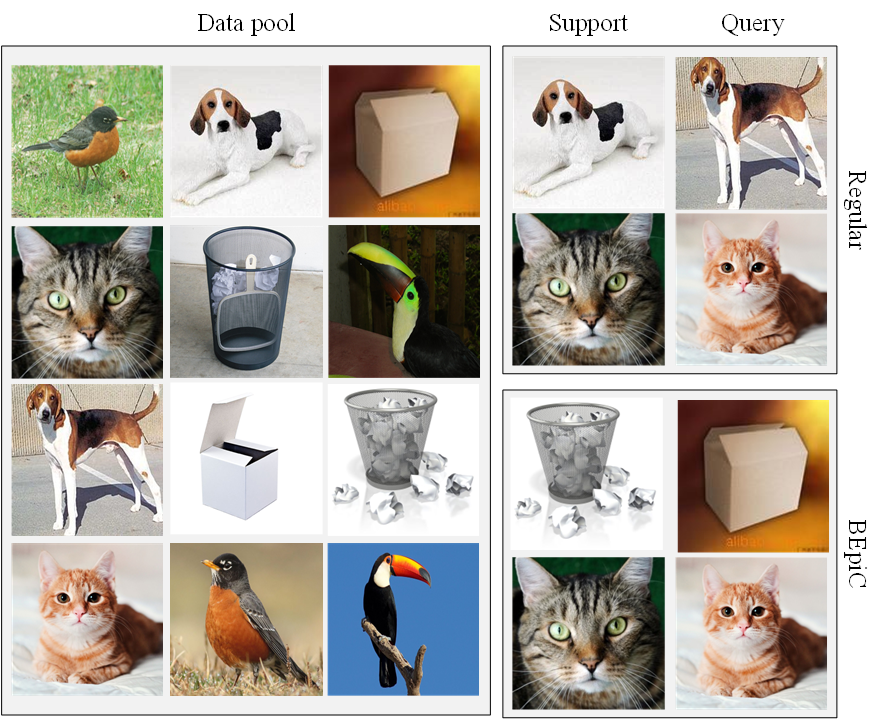
\includegraphics[width=0.9\columnwidth]{FIGURES/bepic/fig.png}
  \caption{Episode generation of Regular and BEpiC from the data pool. In BEpiC, we select the most dissimilar samples.}
  \label{fig:fig}
\end{figure*}

\subsubsection{Samples Selection}

Since the goal of the episode generation is to diversify the samples, sample selection identifies samples that maximize the inter-class distance, which is one of the contributions of our paper. However, computing the distance between every sample across different classes poses a substantial computational challenge, especially for large datasets. To address this, we employ a strategy of randomly designing multiple episodes. For instance, considering a class (referred to as the "cat" class for clarity), we determine which mixture of other classes would yield the most dissimilar set.

The sample selection process involves calculating the centroid of each episode cluster. It is achieved through PCA for dimensionality reduction and mean calculation to determine the centroid. The Euclidean distance metric is then applied to identify the sample closest to the centroid, which is subsequently designated as the class representative. To streamline computations, we later only compare the most centroid images with the ones from the "cat" class. This strategic reduction in the number of comparisons contributes to managing the computational complexity of analyzing large datasets.

We employ the ORB feature-matching algorithm to assess the dissimilarity between samples from the two classes. We select the one with the highest dissimilarity score from a pool of numerous samples. In cases where multiple outputs exhibit the same lowest dissimilarity, we prioritize the first one on the list. This approach ensures we pinpoint the most dissimilar pair of samples, effectively identifying representative class instances. In the following subsection, we provide a brief description of PCA and ORB.

\textbf{PCA:}  Given a dataset \( {X} \in \mathbb{R}^{n \times p} \) with \( n \) observations and \( p \) variables, PCA seeks to find a set of orthogonal vectors, that capture the most variance in the data. The first step in PCA is to subtract the mean of each variable from the dataset \( {X} \), resulting in,

\begin{equation}
{X}_{\text{centered}} = {X} - \bar{{X}}
\end{equation}

Next, we compute the covariance matrix using the center,

\begin{equation}
 {C} = \frac{1}{n-1} {X}_{\text{centered}}^T {X}_{\text{centered}}
\end{equation}

We solve \( {C} {V} = {V} {\Lambda} \) to get eigenvectors \( {V} \) and eigenvalues \( {\Lambda} \) and project the data onto the new coordinate system \( {Y} = {X}_{\text{centered}} {V} \). We select the top \( k \) eigenvectors to reduce the dataset dimensionality: \( {Y}_k = {X}_{\text{centered}} {V}_k \).

The variance explained by the \( i \)-th principal component is \( \frac{\lambda_i}{\sum_{j=1}^p \lambda_j} \), where \( \lambda_i \) is the \( i \)-th eigenvalue.

\textbf{ORB:} ORB calculates the angle intensity based on its center offset, making it suitable for determining orientation., given by
\begin{equation} \label{eq:moment}
\mathrm{m}_{pq}=\sum_{x,y}{x}^{p}{y}^{q}I(x,y)
\end{equation}
where $m$ is referred to as the moment patch, $p$ and $q$ are the sequences of moments comparable to mechanical moments, and $(x, y)$ is the pixel coordinate keypoint of image, $I$. The centroid can then be determined using the moment in \eqref{eq:moment} as
\begin{equation}
C = \left(\frac{m_{10}}{m_{00}},\frac{m_{01}}{m_{00}} \right)
\end{equation}

The centroid will be located using the image's pixel matrix, designated as $\{m_{00}, m_{01}, \cdots\}$. The vector is created by connecting the centroid $C$ with the angle's center. In other words, the patch's orientation can be computed as:

\begin{equation}
\Theta_{orient}=arctan(m_{01},m_{10})
\end{equation}

where $\Theta_{orient}$ is the orientation angle based on the gradients. These selected samples craft the BEpiC episodes using any dataset that contains numerous classes.

\subsection{Dataset}
We conduct experiments on two popular datasets in meta-learning, Caltech 256 \cite{griffin_holub_perona_2022} and miniImageNet \cite{liu2020embarrassingly}. The statistics for the two datasets can be found in Table \ref{table:data}.

\begin{table*}[!ht]
    \centering
    \caption{Statistics from the two image datasets.}
    \begin{adjustbox}{width=0.9\linewidth}
    \renewcommand{\arraystretch}{1.5} 
    \begin{tabular}{|l|l|l|l|l|l|l|}
    \hline
        \textbf{Dataset} & \textbf{\#Classes} & \textbf{\#Training} & \textbf{\#Validation} & \textbf{\#Test} & \textbf{\#Total samples} & 
        \textbf{\#Samples/Class} \\ \hline
        Caltech 256 & 256 & 150 & 56 & 50 & 30,607 & at least 80 \\ \hline
        miniImageNet & 100 & 64 & 16 & 20 & 60,000 & 600 \\ \hline
    \end{tabular}
    \end{adjustbox}
\label{table:data}
\end{table*}

\subsubsection{Caltech 256} The Caltech 256 dataset is considered an enhancement over its predecessor, the Caltech 101 dataset, due to features such as larger category sizes and the inclusion of new and more extensive clutter categories \cite{li_andreeto_ranzato_perona_2022}. This dataset is ideal for developing visual recognition and classification models, comprising 30,607 real-world images across 257 classes of varying sizes (256 object classes plus an additional clutter class). Each class includes 100 training images and 20 test images.

\subsubsection{miniImageNet} miniImagenet, a subset derived from the extensive ImageNet dataset, is specifically tailored for few-shot learning tasks. The unique challenge posed by miniImagenet lies in its demand for machine learning models to generalize effectively with only a limited number of training examples. This dataset consists of 100 classes, each accompanied by 600 images. We allocate 64 classes for training, 16 classes for validation, and 20 classes for testing. This division ensures a balanced distribution of classes across different sets, enabling a comprehensive assessment of model performance.

The experimental evaluation and results are presented in the next sections, which employ the sampling process and dataset.

\subsection{Experimental Evaluation}

We conducted a comprehensive evaluation of our model, focusing on its test accuracy to ensure a thorough examination of its performance. We extended our analysis to encompass the accuracy of various model configurations. The evaluation employed terminologies commonly used in meta-learning research, specifically the $n$-way $k$-shot learning framework, where $n$-way denotes the number of classes and $k$-shot indicates the number of samples the classifier encounters in each training episode. 

For binary classification, the number of ways is fixed as 2-way. However, we vary the $k$-shot classification to explore different configurations with $1, 5, 20$ values. Across all experiments, the total number of epochs is set at $10$, each comprising $10,000$ training episodes and $100$ test episodes.

For every input, the image size is standardized to $(84, 84, 3)$, ensuring uniformity in the dataset preprocessing. This consistent approach to experimental design allows for a thorough investigation of the model's performance under distinct $k$-shot scenarios, shedding light on its adaptability and effectiveness in binary classification tasks.


We experimented with two configurations: 1. exclusively utilizing the BEpiC setup and, 2. incorporating both BEpiC and Regular setups for episode generation. Our findings indicate that the BEpiC configuration exhibits superior generalization compared to the sole use of regular task generation. Moreover, a significant performance enhancement is observed when combining BEpiC with the Regular setup, particularly with increased episodes and shots in each task.

Table \ref{table:bepiC} provides insights into the classifier's performance on the BEpiC test set, where the test class comprises samples from the most dissimilar classes. On the other hand, Table \ref{table:reg+bepiC} outlines the classifier's performance on the BEpiC test set in conjunction with the Regular test data. Lastly, Table \ref{table:random} provides the classifier's performance on random test sets, where both the training and test sets were designed randomly without adhering to our proposed method, implying that the largest inter-class distance was not a focal consideration. These comparative tables underscore the effectiveness and advantages of our proposed approach.

\begin{table}[!ht]
\centering
\caption{Performance of the classifier on the BEpiC test dataset.}
\begin{adjustbox}{width=0.7\linewidth}
\renewcommand{\arraystretch}{1.5} 
\begin{tabular}{|l|l|l|l|l|l|l|}
 \hline
\multirow{3}{*}{\textbf{Train methods}} & \multicolumn{6}{c|}{\textbf{Test accuracy (\%)}}                         \\  \cline{2-7}
                               & \multicolumn{3}{c|}{\textbf{Caltech 256}} & \multicolumn{3}{|c|}{\textbf{miniImageNet}} \\ \cline{2-7}
                               & \textbf{1-shot}  & \textbf{5-shot}  & \textbf{20-shot} & \textbf{1-shot}    & \textbf{5-shot}   & \textbf{20-shot}   \\  \hline
Regular                        & 60.50    & 70.90    & 81.05   & 63.50      & 70.80     & 75.25     \\  \hline
BEpiC                          & \textbf{61.00}      & \textbf{71.90}    & \textbf{81.50}    & \textbf{64.00}        & \textbf{71.00}       & \textbf{76.66}     \\  \hline
Regular+BEpiC                  & \textbf{63.50}    & \textbf{72.80}    & \textbf{81.80}    & \textbf{65.00}        & \textbf{71.40}     & \textbf{76.66}    \\  \hline
\end{tabular}
\end{adjustbox}
\label{table:bepiC}
\end{table}

\begin{table}[!ht]
\centering
\caption{Performance of the classifier on the Regular+BEpiC test dataset.}
\begin{adjustbox}{width=0.7\linewidth}
\renewcommand{\arraystretch}{1.5} 
\begin{tabular}{|l|l|l|l|l|l|l|}
 \hline
\multirow{3}{*}{\textbf{Train methods}} & \multicolumn{6}{c|}{\textbf{Test accuracy (\%)}}                         \\  \cline{2-7}
                               & \multicolumn{3}{c|}{\textbf{Caltech 256}} & \multicolumn{3}{|c|}{\textbf{miniImageNet}} \\ \cline{2-7}
                               & \textbf{1-shot}  & \textbf{5-shot}  & \textbf{20-shot} & \textbf{1-shot}    & \textbf{5-shot}   & \textbf{20-shot}   \\  \hline
Regular                        & 61.00    & 70.00    & \textbf{81.50}   & 65.50  & 69.60     & 76.46     \\  \hline
BEpiC                          & \textbf{62.00}    & \textbf{70.40}  & 80.96  & 65.00    & \textbf{70.50}     & \textbf{76.70}     \\  \hline
Regular+BEpiC                  & \textbf{63.00}    & \textbf{71.97} & 81.25  & \textbf{67.00}    & \textbf{71.00}       & \textbf{76.83}    \\  \hline
\end{tabular}
\end{adjustbox}
\label{table:reg+bepiC}
\end{table}

\begin{table}[!ht]
\centering
\caption{Performance of the classifier on the random test dataset.}
\begin{adjustbox}{width=0.8\linewidth}
\renewcommand{\arraystretch}{1.5} 
\begin{tabular}{|l|l|l|l|l|l|l|}
 \hline
\multirow{3}{*}{\textbf{Train methods}} & \multicolumn{6}{c|}{\textbf{Test accuracy (\%)}}                         \\  \cline{2-7}
                               & \multicolumn{3}{c|}{\textbf{Caltech 256}} & \multicolumn{3}{|c|}{\textbf{miniImageNet}} \\ \cline{2-7}
                               & \textbf{1-shot}  & \textbf{5-shot}  & \textbf{20-shot} & \textbf{1-shot}    & \textbf{5-shot}   & \textbf{20-shot}   \\  \hline
Regular                        & 57.50    & 70.70    & 80.70   & 62.40  &  \textbf{70.20}    &   74.83   \\  \hline
BEpiC (random)                          & \textbf{58.00}    & \textbf{71.00}  & \textbf{81.25}  & \textbf{63.70}    & 70.10     & \textbf{75.33}     \\  \hline
Regular+BEpiC (random)                  & \textbf{61.00}    & \textbf{71.30} & \textbf{81.50}  & \textbf{64.90}    & \textbf{71.16}       & \textbf{76.23}    \\  \hline
\end{tabular}
\end{adjustbox}
\label{table:random}
\end{table}

\subsection{Results and Discussion} \label{results}

The findings from Table \ref{table:bepiC} provide compelling evidence supporting the superiority of BEpiC over Regular episodes in 1-shot classification scenarios. In this context, where test samples encompass any two different categories from the real world, our proposed MAML training method consistently outperforms the conventional approach for both datasets. The subsequent amalgamation of Regular and BEpiC setups results in a noteworthy 2\% and 1.5\% improvement in accuracy for 1-shot classifications on both datasets. This enhancement can be attributed, in part, to the doubled sample size, indicating that the classifier operates more effectively on the intended test samples in this combined arrangement. Expanding the evaluation to 5-shot and 20-shot classifications reveals a consistent trend, with Regular+BEpiC achieving the highest accuracy in all cases for both Caltech 256 and miniImageNet datasets.

The insights from Table \ref{table:reg+bepiC} introduce intriguing nuances to our analysis. In the context of Caltech 256, including Regular test samples alongside BEpiC samples led to a 0.5\% improvement in accuracy for the Regular classifier in 1-shot classification. This improvement is intuitively understandable, as adding Regular test samples facilitated the Regular setup's classification task. Surprisingly, the MAML classifier tested on BEpiC and Regular test samples achieved 1\% higher accuracy than the previous BEpiC-only output. This seemingly counterintuitive result is clarified by recognizing the reduced challenge in classifying Regular test samples due to minimal intra-class distance. Consequently, the classifier excelled in handling Regular samples alongside BEpiC samples, resulting in higher accuracy. Notably, the 20-shot Regular Caltech 256 classification achieved the highest accuracy in this setup, suggesting that Regular test samples favored the Regular approach in achieving higher accuracy in 20-shot scenarios. However, for 5-shot learning, a drop in accuracy across all classifiers indicates the proposed method's increased suitability when there is greater variety in test samples. For miniImageNet, Regular+BEpiC consistently achieved the highest accuracy, except in 1-shot scenarios where BEpiC achieved slightly lower accuracy, with Regular achieving a 0.5\% advantage.

Table \ref{table:random} serves as a cautionary demonstration of the repercussions of disregarding the proposed method. The outputs reveal the necessity of our proposed approach by employing random samples for training episodes, irrespective of their inter-class distance, and testing with a BEpiC setup using random samples. Lower accuracy in 1-shot learning across all outputs compared to Table \ref{table:bepiC} reinforces the importance of strategically selecting samples with higher inter-class distance. This trend persists in 20-shot and 5-shot Caltech 256 scenarios. However, in 5-shot miniImageNet, Regular training outperforms BEpiC (random), affirming the suitability of our proposed method, mainly when training on BEpiC samples with significant intra-class distance.

In summary, the evidence presented consistently advocates for the effectiveness of the proposed BEpiC methodology. Regular+BEpiC emerges as a robust approach, showcasing superior performance across various few-shot learning scenarios compared to conventional and random training methods.

\subsection{Ablation Study}

In our investigation of classifier performance, we systematically varied the number of clusters for the negative class to discern its impact. The choice of cluster count plays a pivotal role in influencing the selection of the most distant samples while considering computational costs. Striking the right balance is crucial for optimizing our research outcomes.

Table \ref{table:5} showcases the classifier's performance with the negative classes drawn from 5 clusters. The results, compared against those from BEpiC in Table \ref{table:bepiC}, are evaluated based on the change in test accuracy (\%). Positive change indicates improved accuracy, while negative values signify a decline. For 5 clusters, there is a consistent drop in test accuracy across all shot learning scenarios, ranging from 0.1\% to 0.66\%. This implies a discernible reduction in classifier performance across various settings when employing 5 clusters.

In Table \ref{table:20}, we extend our analysis to 20 negative class clusters, observing a mixed performance outcome. While some scenarios show improvement, others exhibit marginal decreases. Factors such as multiple clusters being equidistant may contribute to the performance fluctuations. The change in accuracy spans from -0.66\% to 0.27\%. However, the absence of consistent accuracy improvement, coupled with a doubling of computational time, leads us to choose 10 clusters as the optimal value.

Our exploration underscores the delicate trade-off between the number of clusters, computational efficiency, and classifier performance. The choice of 10 clusters emerges as a judicious compromise, balancing enhancing accuracy and managing computational costs in our research endeavors.

\begin{table}[!ht]
\centering
\caption{Performance of the classifier on the random test dataset.}
\begin{adjustbox}{width=0.75\columnwidth}
\renewcommand{\arraystretch}{1.5} 
\begin{tabular}{|l|l|l|l|l|l|l|}
 \hline
\multirow{2}{*}{\textbf{5 Clusters} }  & \multicolumn{6}{c|}{\textbf{Test accuracy (\%)}}                             \\
\cline{2-7}
                            & \multicolumn{3}{c|}{\textbf{Caltech 256}} & \multicolumn{3}{c|}{\textbf{miniImageNet}} \\ \cline{2-7}
                            & \textbf{1-shot}   & \textbf{5-shot}   & \textbf{20-shot}   & \textbf{1-shot}   & \textbf{5-shot}   & \textbf{20-shot}   \\ \hline
BEpiC                     & 60.72    & 71.32    & 81.30      & 63.67     & 70.90     & 76.00        \\ \hline
(\%) change                & -0.28    & -0.58    & -0.20      & -0.33     & -0.10     & -0.66    \\ \hline
\end{tabular}
\end{adjustbox}
\label{table:5}
\end{table}

\begin{table}[!ht]
\centering
\caption{Performance of the classifier on the random test dataset.}
\begin{adjustbox}{width=0.75\columnwidth}
\renewcommand{\arraystretch}{1.5} 
\begin{tabular}{|l|l|l|l|l|l|l|}
 \hline
\multirow{2}{*}{\textbf{20 Clusters} }  & \multicolumn{6}{c|}{\textbf{Test accuracy (\%)}}                             \\
\cline{2-7}
                            & \multicolumn{3}{c|}{\textbf{Caltech 256}} & \multicolumn{3}{c|}{\textbf{miniImageNet}} \\ \cline{2-7}
                            & \textbf{1-shot}   & \textbf{5-shot}   & \textbf{20-shot}   & \textbf{1-shot}   & \textbf{5-shot}   & \textbf{20-shot}   \\ \hline
BEpiC                     & 61.16    & 71.83    & 81.67      & 64.11     & 71.27     & 76.00        \\ \hline
(\%) change               & 0.16    & -0.07    & 0.17      & 0.11    & 0.27     & -0.66    \\ \hline
\end{tabular}
\end{adjustbox}
\label{table:20}
\end{table}

\subsection{Conclusion and Future Work} \label{conclusion}

This study introduces a novel episode generation strategy for binary classification tasks that distinguish between positive and negative classes and comprise various samples. The proposed approach leverages statistical analysis to curate training episodes, emphasizing samples with the highest inter-class distance. The results underscore the proposed method's robustness in effectively identifying test samples using BEpiC episodes. Across all scenarios, the proposed method consistently outperforms classifiers trained through conventional methods, showcasing superior accuracy.

An additional enhancement to the proposed methodology involves the integration of BEpiC with Regular training samples. This hybrid approach adds robustness to the classifiers and improves accuracy. The findings emphasize the potential of combining different training setups to achieve superior performance in binary classification tasks.

This study aims to extend the classifier's capabilities to handle multi-class classification scenarios as part of future work. Additionally, efforts will be directed toward contributing to the evolution of the classifier's architecture to mitigate any overfitting issues. These advancements are expected to broaden the applicability and effectiveness of the proposed meta-learning strategy, fostering its utility in diverse classification tasks.

\section{Task 2: MetaRep: Improving Meta-Learning Accuracy by  Learning Episodic Representation}

\subsection{Introduction}

Traditional machine learning (ML) algorithms require massive datasets to reach their peak performance. In addition, these algorithms also suffer if the test domain slightly deviates from the training domain. Above all, if a new class is introduced, it requires retraining from scratch. On the other hand, human learning is far more advanced as people can learn from only a few samples and distinguish a new class without seeing many examples. This is because humans use their previous experience to learn a new task. Meta-learning, a relatively new branch of  ML,  mimics this process to bridge the gap between ML and human learning with fewer data from different domains  \cite{such2017deep}.

Most meta-learning algorithms \cite{vinyals2016matching,li2017meta,nichol2018reptile,setlur2020support} are centered around the concept of "learning-to-learn," which involves generating tasks or episodes to discern patterns from a limited number of samples. This process entails the training and testing phases, where the samples are partitioned into support and query sets \cite{bennequin2021bridging}. The support set aids in comprehending class representations, while the query set is utilized for inference. To train a meta-learner, batches of data (episodes in meta-learning) are generated by sampling the training data. Therefore, during training, meta-learning algorithms are exposed to a variety of classes that may not be present in the test classes. This allows ample opportunity to incorporate more classes into the training process. However, existing meta-learning approaches fail to fully exploit the potential of abundant training samples to learn episodic representations without label information \cite{hospedales2021meta}. This limitation stems from their reliance on labeled support sets for task adaptation. Moreover, these approaches are primarily designed around supervised learning principles, where labeled samples are necessary for learning \cite{zhang2023learning}. Consequently, the rich diversity in unlabeled data remains unused. To overcome this limitation, a more flexible representation-learning strategy is required that effectively integrates unlabeled data into the episodic learning process to improve model adaptability and performance \cite{tian2020rethinking}.

Representation learning is a widely established way \cite{9770283, 9363924} of boosting classification accuracy in a low-data regime. Typically, representation learning unfolds in two stages  \cite{chen2020simple, grill2020bootstrap}: unsupervised representation learning followed by supervised learning applied to the acquired parameters. However, in the context of meta-learning, where episodes are pivotal, the conventional representation learning approaches designed for batch learning may not be directly implemented in meta-learning. 

To address this challenge, we introduce MetaRep, a representation-learning approach tailored specifically for meta-learning to capture episode-specific representations. MetaRep leverages distinct image augmentation techniques to construct training episodes using unlabeled data. Support sets are formed by randomly sampling from the data pool, and image augmentation techniques are applied to generate query sets. Technically, it works for datasets like Omniglot \cite{lake2015human} and mini-Imagenet \cite{ILSVRC15} or larger datasets because they contain a multitude of samples and classes. Therefore, we hypothesize that the probability of drawing from the same class is insignificant.

MetaRep consists of two steps of training. In the first step, we apply the fully unsupervised training to learn the latent representations of the dataset. Throughout this phase, we utilize the labeled test sets to monitor performance. While the accuracy achieved during unsupervised representation learning may not rival that of supervised learning, the meta-learning algorithm still manages to achieve some degree of accuracy.  Although unsupervised representation falls behind supervised learning accuracy, it is a good initialization point to boost supervised learning performance. Hence, in the second step, we utilize the learned parameters from the unsupervised learning model to initialize the supervised meta-learning process rather than resorting to random initialization. This strategic use of pre-learned parameters effectively transforms the entire process into a semi-supervised meta-learning algorithm \cite{sun2019meta}, thereby enhancing performance.

In addition, MetaRep employs data augmentation to increase learning effectiveness. For an effective augmentation technique, we drew inspiration from SimCLR \cite{chen2020simple} and combined it with color invert and random flip augmentations. This makes the MetaRep model agnostic and adaptable to various meta-learning models. 

To experimentally validate the effectiveness of MetaREP, we evaluated its performance across two prominent meta-learning architectures: Model-Agnostic Meta-Learning (MAML) \cite{finn2017model} and Relation Network (RN) \cite{sung2018learning}. In our experiments, we introduced a modification to the MAML network architecture by integrating temperature \cite{sohn2016improved} into the SoftMax activation function in the inner loop. This adjustment was aimed at mitigating overfitting during unsupervised training. While we retained the RN architecture unchanged, we optimized our hyperparameters and architecture to achieve higher accuracy compared to the results reported in \cite{sung2018learning}. Our experimentation shows that the proposed MetaRep method can enhance the accuracy of any state-of-the-art meta-learning model.

While our approach incorporates techniques like data augmentation and temperature scaling, MetaRep's novelty lies in its unique adaptation for episodic representation learning. Our data augmentation strategy combines methodologies with episodic-specific modifications, creating query samples with demonstrably distinct feature distributions—as verified through our histogram analysis showing entirely new pixel intensities in each run. Unlike previous approaches that produce similar augmented samples, our method introduces meaningful uncertainty between episodes, critical for effective meta-learning where samples may appear across multiple episodes. Complementing this, our introduction of temperature-scaled SoftMax specifically in the meta-learning inner loop addresses the overfitting challenge in unsupervised episodic learning, significantly improving accuracy by forcing the model to learn more discriminative features. Together, these technical innovations enable MetaRep to effectively bridge supervised and unsupervised paradigms by learning transferable episodic representations without labels—representing a fundamental shift from both standard meta-learning approaches that require labeled data for episodic learning and traditional representation learning techniques that aren't optimized for episodic adaptation.

\subsection{Contributions}

Our key contributions are as follows:
\begin{itemize}
    \item We introduce MetaRep, a novel semi-supervised meta-learning framework that leverages unsupervised representation learning to enhance meta-learning performance. Our approach demonstrates significant accuracy improvements across multiple architectures while reducing dependency on labeled data.
    
    \item We develop an enhanced data augmentation strategy that combines SimCLR methodologies with targeted modifications for meta-learning scenarios. Through empirical analysis and visualization, we show how our augmentation technique generates more diverse and informative query sets, leading to improved representation learning.
    
    \item We propose a temperature-scaled adaptation of MAML's inner loop optimization, effectively addressing the overfitting challenges in unsupervised meta-learning. This modification, combined with our optimized implementation of Relation Networks, achieves state-of-the-art performance on standard few-shot learning benchmarks.
    
    \item We validate MetaRep's model-agnostic properties through extensive experimentation across multiple architectures and datasets. Our empirical results demonstrate both cross-architecture adaptability and strong transfer learning capabilities, with MetaRep maintaining consistent performance improvements even when training with significantly reduced labeled data. These results establish MetaRep as a robust, general-purpose enhancement for meta-learning systems.
    
\end{itemize}

\subsection{Related Work}

Meta-learning \cite{hospedales2021meta} has found extensive applications across diverse domains, including self-driving cars, face recognition, and computer vision. While primarily aimed at enabling classification with minimal samples, meta-learning models typically require substantial labeled data for training. This has increased interest in data augmentation techniques within the meta-learning community. Yao et al. \cite{yao2021improving} introduced task augmentation methods, MetaMix and channel shuffle, effectively reducing overfitting by linearly combining features and labels or randomly shuffling channels across classes. Rajendran et al. \cite{rajendran2020meta} proposed a meta-augmentation framework based on information theory to enhance generalization by introducing controlled randomness. However, both approaches remain supervised and still depend significantly on labeled data.

Recent advancements in implicit semantic data augmentation (ISDA) have offered promising alternatives for augmenting training data. Wang et al. \cite{wang2019implicit, wang2021regularizing} proposed ISDA techniques, leveraging semantic transformations within deep feature spaces to efficiently augment datasets and improve model generalization. Their methods implicitly augment data by minimizing upper bounds on the expected loss, significantly enhancing the generalization capabilities of deep networks with minimal computational overhead.

Hsu et al. \cite{hsu2018unsupervised} developed one of the earliest unsupervised meta-learning methods called CACTUs, assigning pseudo-labels through nearest neighbor clustering. Despite its effectiveness, CACTUs is computationally expensive due to additional embedding learning and clustering steps \cite{hartigan1979algorithm}. Moreover, its unsupervised nature limits its accuracy compared to supervised approaches.

Semi-supervised learning has become an active area of research, addressing challenges like limited labeled data and noisy labels. Recent frameworks, such as SimCLR \cite{chen2020simple}, C2MT \cite{zhang2024cross}, and PSSCL \cite{zhang2025psscl}, have proposed advanced strategies for handling limited data and noisy labels. Zhang et al. \cite{zhang2024cross} introduced the cross-to-merge training (C2MT) framework, leveraging cross-training of two networks and balanced data partitioning. PSSCL \cite{zhang2025psscl} focuses on progressively selecting and refining clean data samples, employing contrastive learning for robust semi-supervised training.

To address challenges in domain adaptation and transfer learning scenarios, recent studies have presented innovative approaches. Xie et al. \cite{xie2024adapting} proposed target-oriented transferable semantic augmentation (\text{$T^{2}SA$}), implicitly generating target-like augmented data to enhance model generalization across domains. Their method utilizes class-wise prototype constraints to ensure discriminative and representative augmentation. Additionally, Du et al. \cite{du2024probabilistic} introduced probabilistic contrastive learning (ProCo), effectively addressing issues arising from long-tailed distributions by efficiently sampling contrastive pairs through probabilistic modeling of feature distributions.

Khodadadeh et al. \cite{khodadadeh2019unsupervised} proposed UMTRA, combining unsupervised meta-learning with augmented query samples within the MAML framework. However, its accuracy remains below supervised methods. Chen et al. \cite{chen2020simple} introduced SimCLR, significantly impacting semi-supervised learning through effective data augmentation and a normalized temperature-scaled cross-entropy loss, motivating our approach toward a semi-supervised meta-learning framework integrating representation and transfer learning.

Other prominent meta-learning methods include MAML \cite{finn2017model}, aiming for rapid adaptation through optimized task embeddings. Variants like Reptile \cite{nichol2018reptile}, Meta-SGD \cite{li2017meta}, and LEO \cite{rusu2018meta} have similarly contributed to the field. The Prototypical Network \cite{snell2017prototypical} introduced a metric space for efficient classification, later surpassed by Relation Networks (RN) \cite{sung2018learning}, which further enhanced accuracy. Oreshkin et al. \cite{oreshkin2018tadam} proposed TADAM, enhancing few-shot learning by task-dependent metric scaling and adaptive metrics, significantly improving classification accuracy on benchmark datasets. Lee et al. \cite{lee2019meta} introduced MetaOptNet, utilizing differentiable convex optimization to leverage linear classifiers as base learners, achieving state-of-the-art results in few-shot learning tasks. In our work, we build upon these methods by modifying MAML and leveraging RN, PN, TADAM and MetaOptNet, emphasizing their model-agnostic nature for improved performance.

Additionally, local supervision methods such as InfoPro \cite{wang2024infopro} have emerged, emphasizing information propagation through gradient-isolated modules. InfoPro maximizes useful information retention while efficiently discarding irrelevant features, providing competitive performance with significant computational efficiency, thus complementing existing meta-learning and semi-supervised frameworks.

\begin{figure}[htbp]
    \centering  
    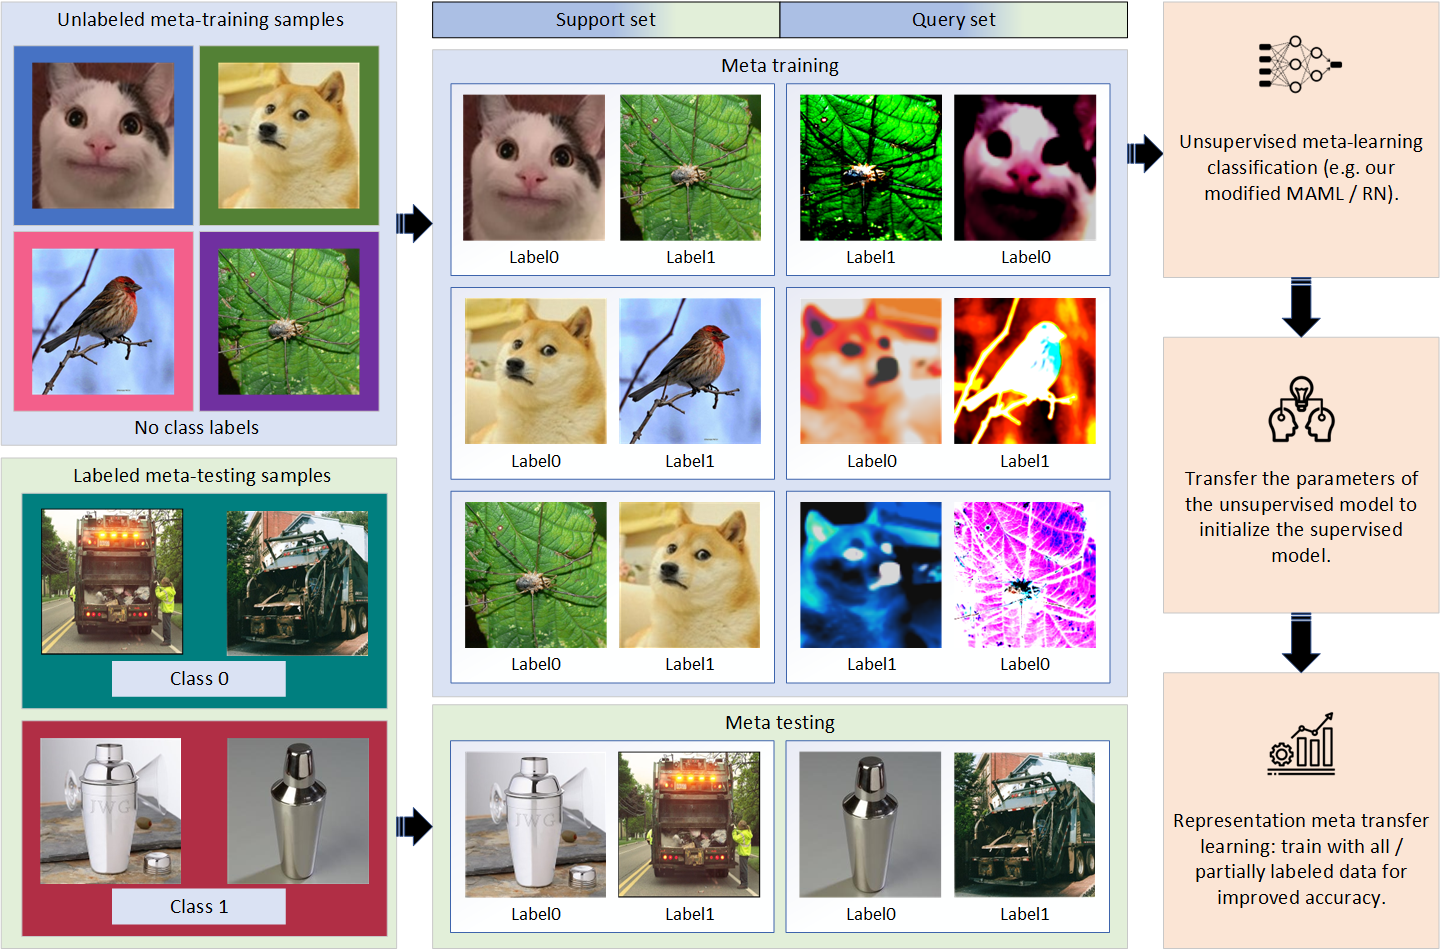
\includegraphics[width=\linewidth]{FIGURES/metarep/corrected.png}
    \caption{Steps of MetaRep, top-left: unlabeled train samples, bottom-left: labeled test samples, middle: episodes for training and testing, middle-left two columns: support set, middle-right two columns: query set, right-top: performing unsupervised meta-learning with the episodes, right-middle: transferring parameters from unsupervised learning to supervised learning, right-bottom: supervised learning with improved accuracy.}
    \label{fig:steps}
  \end{figure}

\subsection{Proposed Method: MetaRep}

In this section, the proposed MetaRep scheme is presented. The MetaRep comprises of two distinct training stages: unsupervised representation learning and semi-supervised meta-learning. A detailed description of each step is presented below. 

\subsubsection{Step 1: Unsupervised Meta-Learning}

\textbf{Data Preparation:} To integrate representation learning with meta-learning, we begin by leveraging either the entire or a subset of the dataset without any label information. Initially, we draw the samples \(x_{n,k}\) from the data pool of \(x_{N}\), where \(n, k\) are the number of ways and the number of shots, respectively, considered in the unsupervised learning and \(N\) is the total number of unlabelled samples. We only design \(n\)-way (or classes), \(1\)-shot support sets because each sample in the support set is drawn randomly, and we cannot randomly add more same-class support samples to that set. However, we can apply data augmentation for the query set to generate multiple query samples of the same class. Subsequently, the effectiveness of generating more query samples is discussed in a later section. 

In episodic learning, every episode sees a combination of new classes. Therefore, after generating the training episodes, assign labeled values \(y_{n,k}\) to each class of the support sets, where \(j\) is the number of ways generated as $\left \{ c_{0},c_{1},...,c_{n-1} \right \}$ and one-hot encoded later. We initialize the random initialization parameter for the unsupervised classifier, $\theta$. We randomly draw the support sets for each task episode and generate the randomly generated support labels. To generate the query set, we pass each sample of the support set through a data augmentation function \(f(A)\) and similarly generate the pseudo labels. Ultimately, we use the regular supervised meta-learning learning test setup to examine the classifier's performance.

\textbf{Deep Dive into Support-Query Set Generation:} We hypothesize that drawing multiple samples from a sizable dataset decreases the likelihood of encountering more than one sample belonging to the same class. Thus, it's imperative to ensure that \(n<<c\) where \(n\) is the number of ways (or the drawn samples, given our 1-shot learning approach) and \(c\) is the total number of classes. However, it is essential to mathematically determine the probability of obtaining unique samples within each class for the datasets used in this study. 

We utilize two distinct datasets: Omniglot and mini-Imagenet. The former typically contains fewer samples per class than the total number of classes, making it highly likely that all drawn samples originate from different classes. Conversely, the mini-Imagenet has more samples (\(600)\) in each class than the total number of classes, resulting in a slightly lower probability of samples originating from different classes. Nonetheless, both datasets feature an equal number of samples per class, denoted as \(m\). Now, we can calculate the probability of the samples belonging to different classes as follows:
\begin{equation}
    P=\frac{c!\cdot m^{n}(c\cdot m-n)}{(c-n)!\cdot (c\cdot m)!}
\end{equation}
\noindent Using the aforementioned formula, the probabilities of 5-way 1-shot classification for the Omniglot (\(1200\) classes) and mini-Imagenet (\(64\) classes) are \(99.21\)\% and \(85.23\)\%, respectively.

Effective data augmentation plays a crucial role in our research, particularly in generating query samples. We combine suggestions from SimCLR \cite{chen2020simple} with additional modifications to enhance effectiveness for RGB image classification, specifically on the mini-Imagenet dataset. The SimCLR paper thoroughly discusses the efficacy of data augmentation and the importance of selecting appropriate augmentation functions, providing valuable insights that guide our approach. They recommend a combination of Gaussian blur, random crop, and random color distortion as the most effective augmentation techniques. Building upon this recommendation, we introduce horizontal flip and random color invert (with a \(50\)\% probability) alongside these three methods. Our experimentation indicates that this augmented combination not only mitigates overfitting but also improves accuracy. Conversely, for the grayscale Omniglot dataset, we solely employ random affine transform. We found that extensive augmentation adversely affects performance, as both support and query samples exhibit significant similarity. Therefore, employing hard augmentation strategies is deemed unnecessary in this particular case.

\textbf{Classifiers:} Our proposed method is model agnostic and can be applied to any model. In this paper, we use two meta-learning models, MAML and RN, to demonstrate the performance on different architectures.  We observe that for MAML, the classifier trained on RGB samples (such as mini-Imagenet in our case) exhibits severe overfitting issues with the regular classifier. This arises because the augmented query samples closely resemble the original support samples, resulting in minimal learning during training. To address this challenge, we introduce a solution by implementing a temperature-scaled SoftMax activation function exclusively within the inner loop of MAML. The inclusion of the temperature term reduces the classifier's confidence in the support set samples, enabling the classifier to gather more information from subtle differences. This adjustment effectively mitigates the overfitting issue, enhancing the performance of MAML. The mathematical expression for temperature-scaled SoftMax is as follows:
\begin{equation}
\frac{\exp(z_{i}/T)}{\sum_{k=0}^{j-1} \exp(z_{k}/T)}
\end{equation}
where the scaling is accomplished by dividing the logits of SoftMax by a value \(T\), known as temperature. \(j\) is the number of ways, and \(z_{i}\), \(z_{k}\) represent the \(i^{th}\), \(k^{th}\) input to the SoftMax, respectively.

We found RN performing counter effectively when using a temperature-scaled SoftMax. We instead used our own set of hyperparameters that led to more improved accuracy than the RN in the original paper.

Following the training of the unsupervised learning algorithm, we preserve the weights and biases for subsequent supervised meta-learning. Consequently, in the classifier of the second step, instead of initializing parameters $\theta$ randomly, we utilize the transferred parameters denoted as $\theta^{*}$. Subsequently, we conduct standard meta-learning procedures to fine-tune and enhance accuracy.

\begin{algorithm}[htbp]
    \caption{MetaRep}
    \label{alg:1}
    \begin{enumerate}
        \item \textbf{Require:} unlabeled dataset $U\{x_N\}$, 
        \item \textbf{Require:} learning rates $\alpha, \beta$, 
        \item \textbf{Require:} augmentation function $f(A)$
        \item Initialize random parameter $\theta$
        \item \textbf{while} not done \textbf{do}
        \begin{enumerate}
            \item Generate episodes $\{x_{n,1}\}$ and create pseudo labels $\{y_{n,1}\}$
            \item \textbf{for each} $(x_{n,1}, y_{n,1})$ \textbf{do}
            \begin{enumerate}
                \item Update the inner loop of meta-learning with custom loss function or hyperparameters
            \end{enumerate}
            \item \textbf{end for}
            \item Update the outer loop of meta-learning with the regular loss function
        \end{enumerate}
        \item \textbf{end while}
        \item Save weights and biases $\theta^*$
        \item \textbf{Input:} Labeled dataset $\{x_{n,k}, y_{n,k}\} \subseteq \{x_{n,1}, y_{n,1}\}$
        \item Initialize $\theta^*$
        \item Perform regular meta-learning steps
    \end{enumerate}
\end{algorithm}

\subsubsection{Step 2: Semi-Supervised Meta-Learning (SSML)}

In this step, we apply SSML within the conventional meta-learning framework, but with parameter initialization from the first classifier. Thus, the transferred parameters originate from the unsupervised meta-learning phase conducted in the initial stage. Let us talk briefly about the two considered classifiers, MAML and RN. Note that we refrain from modifying the SoftMax activation function of MAML at this stage, as the supervised MAML is less prone to overfitting.

\textbf{MAML:} MAML tries to find the optimal parameters $\theta$ derived from a few parametric models $f_{\theta }$. In MAML, we generate the episodes from the data distribution such as $\tau_{i}=(D^{\textrm{tr}},D^{\textrm{val}})$. We use the gradient update to update the initialize parameter $\theta$ to $\theta_{i}^{'}$  across tasks sampled from $p(\tau)$ and is obtained as follows:
\begin{equation}
\theta_{i}^{'}=\theta -\alpha \nabla_{\theta}\pounds_{\tau_{i}}(f_{\theta})
\end{equation}
\noindent where $\alpha$ is the learning rate of the meta-inner loop, and $\pounds$ is the loss function.
In the outer loop of meta-learning, the optimization is performed across tasks via stochastic gradient descent (SGD) to update the $\theta$. It is obtained as follows:
\begin{equation}
\theta\leftarrow \theta -\beta \nabla_{\theta }\sum_{\tau_{i}\sim p(\tau)}\pounds_{\tau_{i}}(f_{\theta^{i}})
\end{equation}
\noindent where $\beta$ is the learning rate of the meta-outer loop.

\textbf{RN:} The main two components of RN are a feature extractor and a relation module. The feature extractor concatenates the features from the support sets, and the query sets as $f_{\varphi}(x_{i})$ and $f_{\varphi}(x_{j})$ through a function $\mathbb{C}(f_{\varphi}(x_{i}),f_{\varphi}(x_{j}))$. 

The combined features are passed through the relation module to obtain their relation score. It is passed through a Sigmoid activation function to obtain the score in a range between 0 to 1. The equation for that is provided below:
\begin{equation}
r_{i,j}=g_{\phi}(\mathbb{C}(f_{\varphi}(x_{i}),f_{\varphi}(x_{j})))
\end{equation}

To create the final output, the relation network's output can also be subjected to extra processing by layers, such as a fully connected neural network. Because of this, the relation network is an adaptable architecture that may be used for various applications. A mean-square-error (MSE) loss function is used to update the network using gradient descent. 
\begin{equation}
\varphi,\phi\leftarrow \arg\min \sum_{i=1}^{m}\sum_{j=1}^{n}(r_{i,j}-1(y_{i}==y_{j}))^{2}
\end{equation}

\textbf{Overall Summary:} The overall method is summarized in this sector with a diagram for better understanding. Figure \ref{fig:steps} depicts the steps of the proposed method. We generate the training episodes from the unlabeled samples. Here, the NT-Xent loss \cite{sohn2016improved} (temperature-scaled SoftMax) is only applied on the MAML for the mini-Imagenet dataset. After training the initial model, we save the parameters and transfer them to the final model for improved performance. Moreover, the pseudo-code for our proposed method is provided in Algorithm \ref{alg:1}.


\textbf{Additional Classifier Architectures:} To comprehensively evaluate MetaRep's model-agnostic capabilities, we implement three additional meta-learning architectures beyond MAML and RN.

\textbf{Prototypical Networks (PN)} \cite{snell2017prototypical} operates by computing class prototypes, the mean feature vector of support samples for each class in an embedding space. Classification is performed by finding the nearest prototype to a query sample using a distance metric (typically Euclidean distance). PN's elegant approach requires no inner loop optimization, making it computationally efficient while maintaining strong performance on few-shot tasks.

\textbf{Task Dependent Adaptive Metric (TADAM)} \cite{oreshkin2018tadam} extends the prototypical network concept by incorporating task conditioning through a Task Embedding Network (TEN). TADAM dynamically adapts its feature extractor for each task using film layers conditioned on task embeddings. Additionally, it employs metric scaling that adjusts the metric space based on task characteristics and leverages auxiliary co-training with standard classification to prevent underfitting. This combination of techniques allows TADAM to achieve superior performance compared to standard meta learning methods.

\textbf{MetaOptNet} \cite{lee2019metaoptnet} frames the inner learning problem as a differentiable convex optimization procedure, specifically using support vector machines (SVMs) for classification. By incorporating this structured classifier rather than a simple linear layer, MetaOptNet leverages the generalization benefits of margin-based classifiers. The SVM's quadratic programming problem is efficiently solved using differentiable optimization techniques, allowing end-to-end training. MetaOptNet is particularly effective in low-data regimes, consistently outperforming other methods on benchmark few-shot classification tasks.

For all three architectures, we apply the MetaRep framework by first learning unsupervised episodic representations, then transferring the learned parameters to initialize supervised meta-learning, following the same procedure as described for MAML and RN.

\subsection{Experiments}

\subsubsection{Data Augmentation for Representation Learning}

We validate our proposed method using two different benchmark datasets in computer vision, Omniglot and mini-Imagenet. Omniglot contains images of handwritten letters from $50$ different languages. This dataset is suitable for few-shot learning because it has $1,623$ characters or classes but only $20$ instances or samples per class. We used $1,200$ classes for training, $100$ classes for validation, and the remaining for testing. In input image dimension to the classifier is $1\times 28\times 28$ pixels, as all are grayscale samples. On the other hand, the mini-Imagenet dataset contains $3\times 84\times 84$ pixels color images. It has a total of $100$ classes, each with $600$ samples. Here, we use $64$ for training, 16 for validation, and $20$ classes for testing.

For selecting the most effective data augmentation, we experimented with different augmentation methods on a trial-and-error basis and found the SimCLR augmentation with an additional augmentation gave the best output for the mini-Imagenet dataset. This section presents the results obtained from various augmentation methods employed in our research. We concentrate on the mini-Imagenet dataset for the augmentation analysis, as the Omniglot dataset typically does not necessitate extensive data augmentation. We also explain why our chosen augmentation works the best for our dataset. Table \ref{tab:unsup} lists the outputs from different augmentation methods using unsupervised learning. Note that all the outputs are obtained by re-implementing different methods using our own hyperparameters, which may provide different results than other literature.

\begin{table}[htbp]
\centering
  \caption{The test accuracy (\%) of unsupervised meta-learning for 5-way 1-shot (5W1S) and 20-way 1-shot (20W1S) classification using mini-Imagenet dataset. For MAML, different temperatures (denoted by ${T}$) are applied in the meta-inner loop.}
 \begin{adjustbox}{width=0.95\linewidth,center}
\tiny
    \begin{tabular}{p{4.5cm}ll|ll}
      \toprule
      \multirow{2}{4.5cm}{\bf Augmentation method} &  \multicolumn{2}{c}{\bf MAML} & \multicolumn{2}{c}{\bf RN} \\
     &  {\bf 5W1S} & {\bf 20W1S} & {\bf 5W1S} & {\bf 20W1S} \\
      \midrule
    \multirow{2}{4.5cm}{Auto augment (UMTRA$^{*}$)}  & 30.1 ($T$=1) & 9.25 ($T$=1) & \multirow{2}{*}{35} & \multirow{2}{*}{9} \\
      & 35.2 ($T$=100) & 11.65 ($T$=10) & &  \\
      \midrule
    \multirow{2}{4.5cm}{Resized crop + Gaussian blur + color distortions (SimCLR)}  & 28.4 ($T$=1)   & 7.6 ($T$=1)   & \multirow{2}{*}{32}   & \multirow{2}{*}{7}  \\
          & 34.4 ($T$=100)    & 11.1 ($T$=10)          &      &   \\
    \midrule
    \multirow{2}{4.5cm}{Horizontal flip (50\%) + color invert (50\%) + resized crop + Gaussian blur + color distortions ({\bf Ours})}    & 33.8 ($T$=1)     & 13.65 ($T$=1)          & \multirow{2}{*}{\bf 39}    &      \multirow{2}{*}{\bf 11.5}     \\
    & {\bf 38.2} ($T$=100)          & {\bf 13.95} ($T$=10)          &          &      \\
      \bottomrule
      $*$re-implementation.
    \end{tabular}
  \end{adjustbox}
  \label{tab:unsup}
\end{table}

\begin{table}[htbp]
  \caption{The test accuracy (\%) of unsupervised meta-learning for 5W1S and 20W1S classification using Omniglot dataset.}
 \begin{adjustbox}{width=\linewidth,center}
\tiny
    \begin{tabular}{p{4.5cm}ll|ll}
      \toprule
      \multirow{2}{4.5cm}{\bf Augmentation method} &  \multicolumn{2}{c}{\bf MAML} & \multicolumn{2}{c}{\bf RN} \\
     &  {\bf 5W1S} & {\bf 20W1S} & {\bf 5W1S} & {\bf 20W1S} \\
      \midrule
    Random transformation + zero pixels (UMTRA$^{*}$) & 48.80 & 24.94 & 61.25 & 35.78 \\
    Resized crop + Gaussian blur (SimCLR) & 48.93 & 27.47 & 66.25 & 43.13  \\
        Random affine transform (30$^{\circ}$) ({\bf MetaRep})  & {\bf 52.83} & {\bf 27.95}  & {\bf 69.12} & {\bf 44.37} \\
      \bottomrule
      $*$re-implementation.
    \end{tabular}
  \end{adjustbox}
  \label{tab:unsup_omni}
\end{table}

From Table \ref{tab:unsup}, we observe the outputs from unsupervised learning for various augmentation functions. Let us begin by discussing the accuracy of MAML. First of all, we use the traditional meta-learning where the temperature parameter in the meta-inner loop for the SoftMax activation function is 1. A temperature of 1 means basically no temperature parameter. For MAML, we discovered that using the optimal temperature in the inner loop increased the accuracy of all the augmentation functions. It is because, when the temperature is 1, the training classifier overfits a lot due to the query set not being very challenging for the support set. When we apply the temperature, the classifier becomes less confident of the classes and can learn more features because of the introduced uncertainty. Initially, we applied the auto-augment function for query sample generation, which achieved slightly higher accuracy than the SimCLR augmentation function in all cases. Our augmentation function achieved 33.8\% and 13.65\% accuracy, which is the highest of all. We introduced temperature parameters as 100 and 10 for 5-way and 20-way, respectively. All the classifiers exhibit improved accuracy for the optimal temperature, and our proposed method obtained the highest accuracy. The temperature is a hyperparameter that shows different performances for different values. In Figure \ref{fig:temp} we illustrated the output accuracy from different temperatures to select the optimal ones. As observed, temperatures 100 and 10 provide the highest accuracy for 5-way and 20-way, respectively.

\begin{figure}[htbp]
    \centering
    \subfloat[\centering 5W1S accuracy for different temperatures.]{{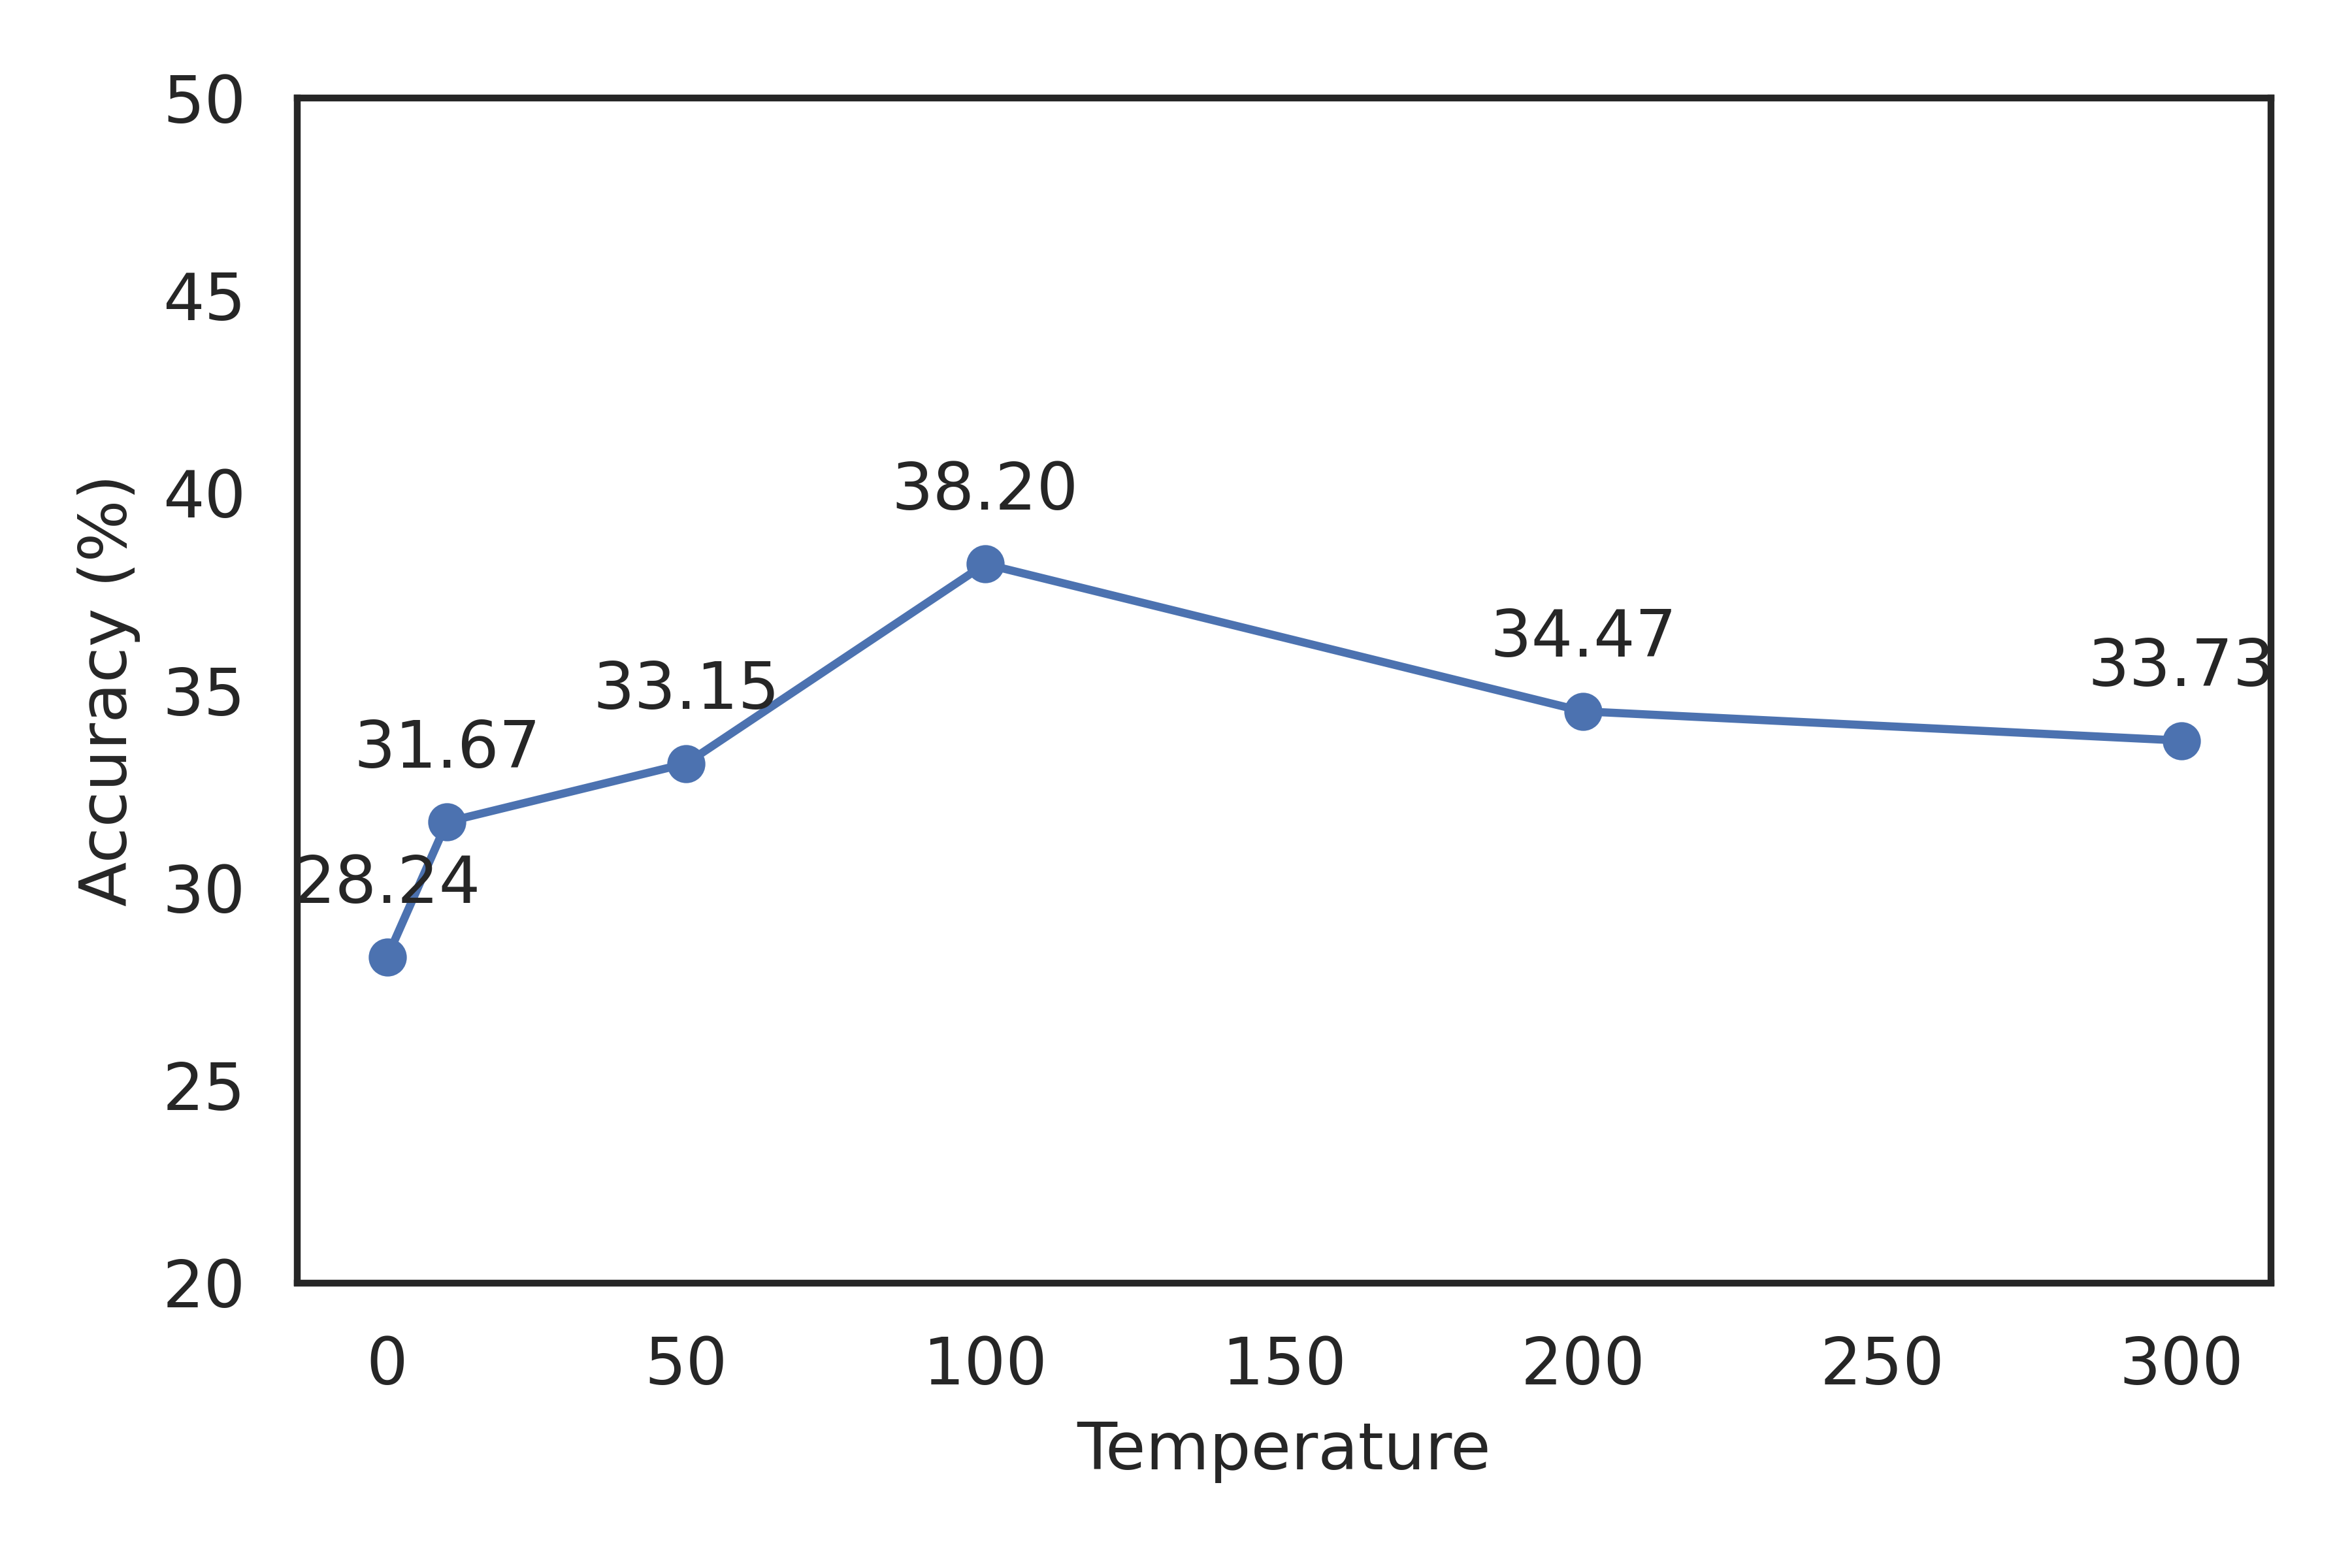
\includegraphics[width=6cm,height=4cm]{FIGURES/metarep/51.png} }}%
    \qquad
    \subfloat[\centering 20W1S accuracy for different temperatures.]{{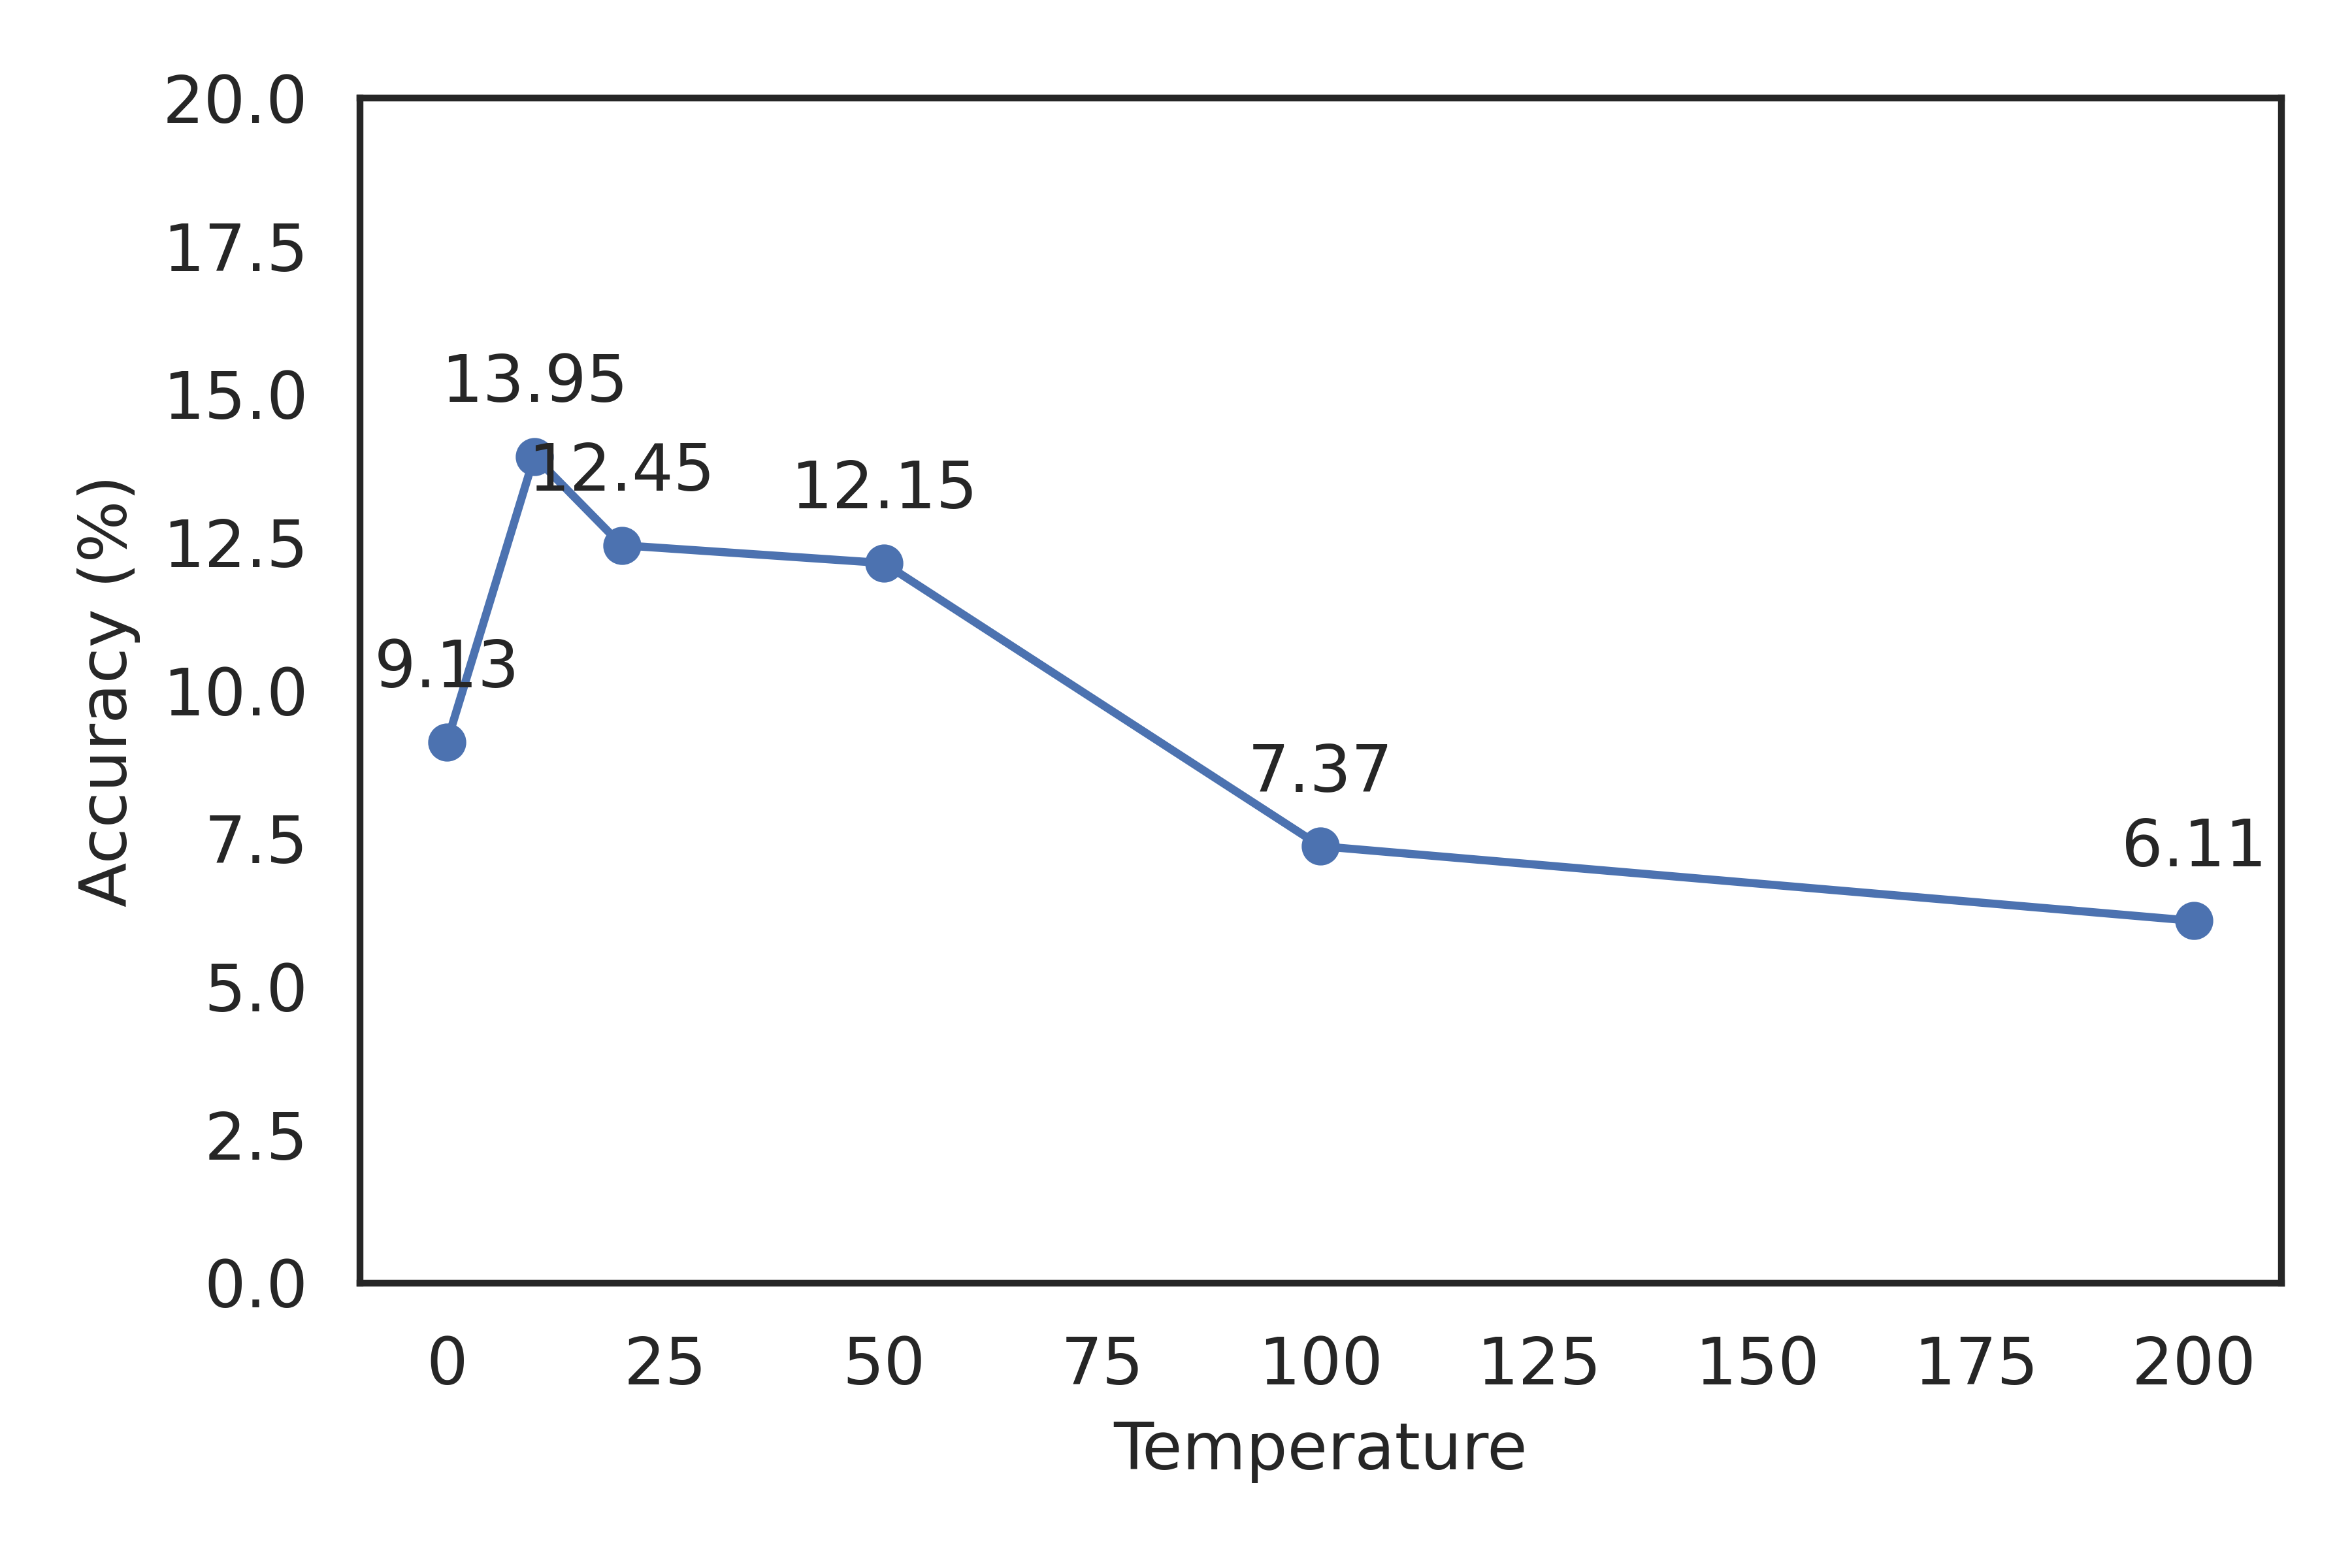
\includegraphics[width=6cm,height=4cm]{FIGURES/metarep/201.png} }}%
    \caption{Effect of different temperatures on test accuracy.}
    \label{fig:temp}
\end{figure}


For the RN, we do not modify anything in the classifier architecture; rather, our motivation is to show that the proposed method is model-agnostic. Nevertheless, our combination of hyperparameters with a ResNet-18 \cite{he2016deep} achieved higher accuracy than MAML for 5-way classification but obtained lower accuracy for 20-way classification. The auto-augment method obtained slightly higher accuracy than the SimCLR augmentation for both 5-way and 20-way classifications. However, SimCLR performs poorly for the 20-way classification and achieves only 7\% accuracy. On the other hand, when we apply our proposed augmentation method, we obtain the highest accuracy for both 5-way and 20-way classifications. Nevertheless, using our proposed method, the RN module achieved higher accuracy than the MAML module for 5-way classification and lower accuracy for 20-way. Therefore, it is evident that the RN unsupervised meta-learning fails to achieve satisfactory accuracy for a higher number of classifications.

We also present the outputs from the Omniglot dataset in Table \ref{tab:unsup_omni} to show the domain adaptability of MetaRep. In Omniglot, the support samples are pretty similar to the query samples. As a result, our experiment found that any hard augmentation on the samples hurt the performance. Therefore, we perform a minimum augmentation to keep the features intact and yet introduce some information in the augmented samples. Moreover, since the samples are grayscale, we could not follow the color distortion function from SimCLR. So, we only applied affine transformation within $30^{\circ}$ to obtain the best transformation. This transformation distorts the samples slightly but keeps the meaning intact. In the case of SimCLR, we only apply resized crop and Gaussian blur as the color distortions do not apply to this dataset. Proof of the effectiveness of our method can be found in the experimental outputs. In this case, the SimCLR augmentation achieved higher accuracy for both MAML and RN in all 5-way 1-shot and 5-way 20-shot classifications. Our proposed method achieves the highest accuracy in all comparisons.

MetaRep can technically be extended to accommodate any n-way 1-shot k-query classification task. This extension is feasible because we have the flexibility to generate different augmented samples in each run for multiple query generation. However, we encountered a drop in accuracy in our proposed model when applied to multiple queries. We attribute this drop in accuracy to the classifier becoming overfit from multiple queries, as they are not distinctly distinguishable. The lack of clear distinctions between multiple query samples likely leads to the classifier being unable to effectively generalize across them, resulting in reduced accuracy. Table \ref{tab:multi-query} represents outputs from MAML for multiple queries. The accuracy drop was significant in all 5-way 5-query and 20-way 5-query shot classifications. Therefore, we do not suggest using our method for a k-query shot. One should instead apply 1-shot unsupervised learning and then transfer the learned parameters to supervised learning. We only applied a 5-way 5-query shot to RN and opted out 20-way 5-query shot because it requires substantial computational resources for a backbone of ResNet-18. In the Omniglot dataset, the accuracy drop for 5-way 5-shot and 20-way 5-shot were 3.68\% and 0.73\% for MAML and 3.87\% and 5.71\% for RN. For mini-Imagenet, the drops are 3.04\% and 1.52\% for MAML and 11\% for RN (N.B. no experiments conducted for 20W1S5Q RN).

\begin{table}[htbp]
  \caption{The test accuracy (\%) and drop of unsupervised MetaRep for n-way, 1-shot multi-query.}
 \begin{adjustbox}{width=\linewidth,center}
\tiny
    \begin{tabular}{p{1.5cm}ll|ll}
      \toprule
      \multirow{2}{1.5cm}{\bf Dataset} &  \multicolumn{2}{c}{\bf MAML} & \multicolumn{2}{c}{\bf RN} \\
     &  {\bf 5W1S5Q} & {\bf 20W1S5Q} & {\bf 5W1S5Q} & {\bf 20W1S5Q} \\
      \midrule
    Omniglot & 49.15 (drop 3.68) & 27.22 (drop 0.73) & 65.25 (drop 3.87) & 38.66 (drop 5.71) \\
    mini-Imagenet & 32.96 (drop 3.04) & 12.43 (drop 1.52) & 28 (drop 11) & N/A \\
      \bottomrule
    \end{tabular}
  \end{adjustbox}
  \label{tab:multi-query}
\end{table}

\begin{figure}[htbp]
  \centering
  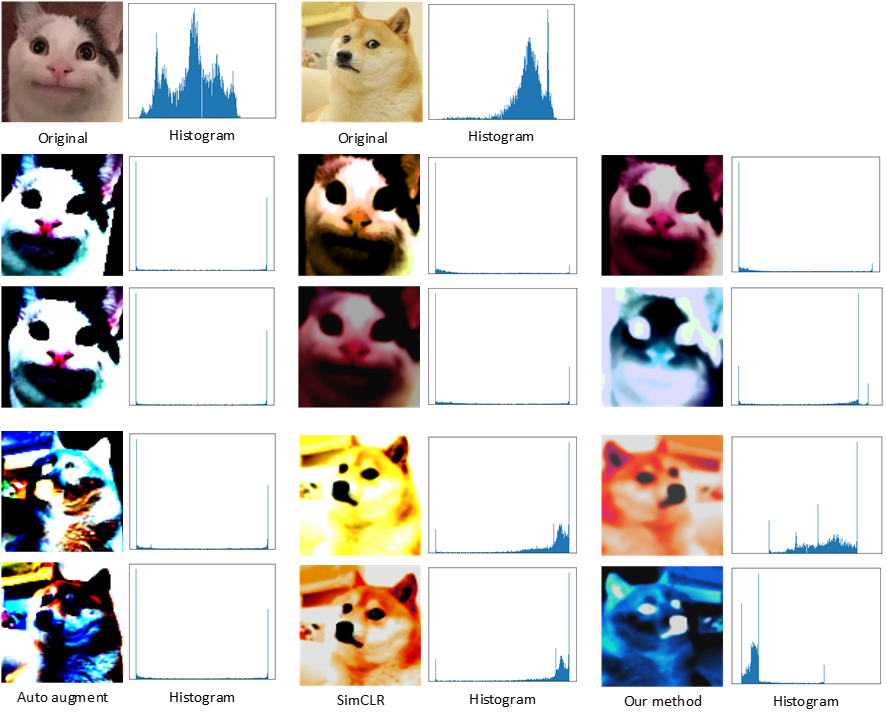
\includegraphics[width=0.8\linewidth]{FIGURES/metarep/figure.png}
  \caption{Histogram of pixel intensities for different augmentation methods.}
  \label{fig:augHist}
\end{figure}

\subsubsection{Computational Resources}

All experiments were conducted using deep learning hardware: a single Nvidia 3080Ti (12GB) GPU for MAML training, and distributed training across two Nvidia 3090Ti (24GB) GPUs plus Google Cloud Platform GPUs for RN, PN, TADAM and MetaOptNet models. Implementation used PyTorch (versions 2.0, 2.3) and Python (versions 3.9, 3.10). For reproducibility, we fixed random seeds to 42, 1234, and 1337 across all experiments.

\subsubsection{Semi-Supervised Meta-Learning (SSML)}

For the second stage, we initialize the meta-learning parameters using weights learned from the unsupervised pre-training phase. To ensure statistical significance, we evaluated all experiments across three random seeds (42, 1234, and 1337). Table \ref{tab:accuracy_omni_mini} presents comprehensive results comparing standard meta-learning approaches with our MetaRep framework across multiple architectures on both Omniglot and mini-ImageNet datasets. All reported accuracies represent means and standard deviations computed across the three independent runs.

Our analysis of Table \ref{tab:accuracy_omni_mini} reveals several important findings across architectures. The baseline model achieves $86.03\pm0.03\%$ on 5W1S1Q for Omniglot, establishing a reasonable lower bound. All meta-learning approaches substantially outperform this baseline, with varying degrees of improvement. 

MetaRep consistently enhances performance across all architectures. For MAML, we observe significant improvements in one-shot learning scenarios (from $93.83\pm0.05\%$ to $96.47\pm0.06\%$ on Omniglot 5W1S1Q), with more modest gains in 5-shot configurations. RN's already strong performance on Omniglot ($99.39\pm0.03\%$ for 5W1S1Q) still improves with MetaRep, reaching perfect $100\%$ accuracy with zero variance. Similarly, PN benefits from MetaRep with accuracy increases from $98.23\pm0.06\%$ to $99.13\pm0.03\%$ on Omniglot 5W1S1Q, and comparable improvements across other configurations.

The advanced architectures TADAM and MetaOptNet also show clear benefits from the MetaRep framework. TADAM's Omniglot performance improves from $99.09\pm0.06\%$ to $100\%$ for 5W1S1Q, while on mini-ImageNet, we observe gains from $57.46\pm0.06\%$ to $58.75\pm0.09\%$. MetaOptNet, despite already achieving optimal performance in several Omniglot configurations, still shows improved consistency in 20W1S1Q (from $98.23\pm0.06\%$ to $99.13\pm0.03\%$) and gains on mini-ImageNet (from $60.36\pm0.09\%$ to $61.23\pm0.06\%$ for 5W1S1Q).

The challenging mini-ImageNet dataset further highlights MetaRep's effectiveness. Across all architectures, we observe consistent improvements: PN ($49.16\pm0.03\%$ to $50.13\pm0.06\%$), MAML ($46.83\pm0.06\%$ to $47.63\pm0.09\%$), RN ($53.03\pm0.06\%$ to $57.03\pm0.09\%$), TADAM ($57.46\pm0.06\%$ to $58.75\pm0.09\%$), and MetaOptNet ($60.36\pm0.09\%$ to $61.23\pm0.06\%$) all benefit from our approach. Particularly noteworthy is RN's substantial 4\% accuracy gain, demonstrating MetaRep's ability to provide more significant benefits to certain architectural paradigms.

The standard deviation values across experiments remain consistently small, indicating the statistical reliability of our results across multiple random seeds. These comprehensive improvements across architectures with different inductive biases strongly validate MetaRep as a truly model-agnostic enhancement to meta-learning frameworks.

\begin{table}[htbp]
  \caption{Classification accuracy (\%) of different methods for random seeds.}
  \centering
  \begin{adjustbox}{width=1.0\linewidth,center}
  \fontsize{9}{9}\selectfont
  \begin{tabular}{p{3cm}cccc|cccc}
  \toprule
  \multirow{2}{*}{\bf Method} & \multicolumn{4}{c|}{\bf Omniglot} & \multicolumn{4}{c}{\bf mini-ImageNet} \\
  & {\bf 1S1Q} & {\bf 5S5Q} & {\bf 20S1Q} & {\bf 20S5Q} & {\bf 1S1Q} & {\bf 5S5Q} & {\bf 20S1Q} & {\bf 20S5Q} \\
  \midrule
  Baseline & $86.03 \pm 0.03$ & $97.67 \pm 0.08$ & $73.03 \pm 0.11$ & $92.37 \pm 0.09$ & $38.47 \pm 0.09$ & $51.23 \pm 0.06$ & N/A & N/A \\
  PN$^{*}$ & $98.23 \pm 0.06$ & $99.13 \pm 0.03$ & $95.63 \pm 0.04$ & $98.53 \pm 0.03$ & $49.16 \pm 0.03$ & $67.86 \pm 0.06$ & N/A & N/A \\
  MAML$^{*}$ & $93.83 \pm 0.05$ & $98.33 \pm 0.06$ & $82.53 \pm 0.06$ & $92.37 \pm 0.06$ & $46.83 \pm 0.06$ & $61.63 \pm 0.03$ & $18.78 \pm 0.09$ & $30.43 \pm 0.06$ \\
  RN$^{*}$ & $99.39 \pm 0.03$ & $100.00 \pm 0.00$ & $97.20 \pm 0.06$ & $99.59 \pm 0.03$ & $53.03 \pm 0.06$ & $64.03 \pm 0.06$ & $24.27 \pm 0.03$ & N/A \\
  TADAM$^{*}$ & $99.09 \pm 0.06$ & $100.00 \pm 0.00$ & $97.57 \pm 0.09$ & $99.69 \pm 0.03$ & $57.46 \pm 0.06$ & $76.27 \pm 0.09$ & N/A & N/A \\
  MetaOptNet$^{*}$ & $100.00 \pm 0.00$ & $100.00 \pm 0.00$ & $98.23 \pm 0.06$ & $100.00 \pm 0.00$ & $60.36 \pm 0.09$ & $76.86 \pm 0.06$ & N/A & N/A \\
  \midrule

  MetaRep PN & $99.13 \pm 0.03$ & $99.73 \pm 0.02$ & $96.23 \pm 0.03$ & $98.77 \pm 0.03$ & $50.13 \pm 0.06$ & $68.41 \pm 0.02$ & N/A & N/A \\
  MetaRep MAML & $96.47 \pm 0.06$ & $98.37 \pm 0.03$ & $83.37 \pm 0.06$ & $92.75 \pm 0.09$ & $47.63 \pm 0.09$ & $61.83 \pm 0.03$ & $18.91 \pm 0.06$ & $30.74 \pm 0.03$ \\
  MetaRep RN & $100.00 \pm 0.00$ & $100.00 \pm 0.00$ & $97.37 \pm 0.06$ & $99.70 \pm 0.03$ & $57.03 \pm 0.09$ & $67.03 \pm 0.06$ & $25.03 \pm 0.06$ & N/A \\
  MetaRep TADAM & $100.00 \pm 0.00$ & $100.00 \pm 0.00$ & $97.90 \pm 0.06$ & $100.00 \pm 0.00$ & $58.75 \pm 0.09$ & $76.94 \pm 0.06$ & N/A & N/A \\
  MetaRep MetaOptNet & $100.00 \pm 0.00$ & $100.00 \pm 0.00$ & $99.13 \pm 0.03$ & $100.00 \pm 0.00$ & $61.23 \pm 0.06$ & $77.11 \pm 0.04$ & N/A & N/A \\
  \bottomrule
  $*$re-implementation.
  \end{tabular}
  \end{adjustbox}
  \label{tab:accuracy_omni_mini}
\end{table}


\begin{table}[htbp]
    \caption{Transferability of MetaRep for different datasets.}
    \begin{adjustbox}{width=0.9\linewidth,center}
    \fontsize{9}{9}\selectfont
    \begin{tabular}{llllll}
    \toprule
    \bf Dataset  & \bf Method    &  \bf 5W1S1Q & \bf 5W5S5Q &  \bf 20W1S1Q & \bf 20W5S5Q \\
    \midrule
    \multirow{6}{*}{CIFAR-FS}       
    & MAML          & $49.63 \pm 0.06$ & $71.23 \pm 0.08$ & $25.79 \pm 0.05$ & $42.19 \pm 0.03$ \\
    & MetaRep MAML  & $53.24 \pm 0.05$ & $71.76 \pm 0.03$ & $26.37 \pm 0.04$ & $42.83 \pm 0.06$ \\
    & RN            & $54.77 \pm 0.04$ & $68.99 \pm 0.05$ & N/A              & N/A              \\
    & MetaRep RN    & $56.08 \pm 0.03$ & $69.70 \pm 0.06$ & N/A              & N/A              \\
    & PN            & $55.36 \pm 0.05$ & $71.67 \pm 0.04$ & N/A              & N/A              \\
    & MetaRep PN    & $57.46 \pm 0.02$ & $73.97 \pm 0.07$ & N/A              & N/A              \\
    \midrule
    \multirow{6}{*}{tieredImageNet} 
    & MAML          & $48.03 \pm 0.04$ & $61.50 \pm 0.05$ & $19.59 \pm 0.06$ & $32.38 \pm 0.03$ \\
    & MetaRep MAML  & $48.23 \pm 0.03$ & $62.07 \pm 0.04$ & $20.13 \pm 0.05$ & $33.26 \pm 0.06$ \\
    & RN            & $51.36 \pm 0.05$ & $67.70 \pm 0.06$ & N/A              & N/A              \\
    & MetaRep RN    & $52.27 \pm 0.04$ & $68.19 \pm 0.03$ & N/A              & N/A              \\
    & PN            & $53.30 \pm 0.06$ & $71.89 \pm 0.05$ & N/A              & N/A              \\
    & MetaRep PN    & $54.68 \pm 0.03$ & $72.07 \pm 0.02$ & N/A              & N/A              \\
    \bottomrule
    \end{tabular}
    \end{adjustbox}
    \label{tab:transfer}
  \end{table}
  
  
\begin{table}[htbp]
    \caption{Accuracy drop (\%) of supervised meta-learning on the partially labeled mini-ImageNet training set.}
    \begin{adjustbox}{width=\linewidth,center}
      \fontsize{9}{9}\selectfont
      \begin{tabular}{p{5cm}llll|llll}
        \toprule
        \multirow{2}{5cm}{\bf Method} 
        & \multicolumn{4}{c|}{\bf 5-way Accuracy} 
        & \multicolumn{4}{c}{\bf 20-way Accuracy} \\
        & {\bf 1S1Q} & {\bf \% Drop} & {\bf 5S5Q} & {\bf \% Drop} 
        & {\bf 1S1Q} & {\bf \% Drop} & {\bf 5S5Q} & {\bf \% Drop} \\
        \midrule
        MAML (50\% labeled data)$^{*}$          & 48.20 & -2.99 & 61.45 & 1.87  & 18.75 & 5.07  & 28.42 & 6.51  \\
        MetaRep MAML (50\% labeled data)        & 49.40 & \textbf{-3.78} & 61.04 & \textbf{1.23}  & 17.94 & \textbf{4.98} & 28.83 & \textbf{6.12} \\
        \midrule
        MAML (25\% labeled data)$^{*}$          & 46.00 & 1.71  & 57.40 & 6.82  & 16.25 & 13.33 & 26.54 & 12.70 \\
        MetaRep MAML (25\% labeled data)        & 47.20 & \textbf{0.84}  & 58.25 & \textbf{5.74}  & 17.50 & \textbf{7.31} & 27.05 & \textbf{11.92} \\
        \midrule
        RN (50\% labeled data)$^{*}$            & 39.00 & 26.42 & 58.20 & \textbf{9.06}   & 19.75 & 18.56 & N/A   & N/A   \\
        MetaRep RN (50\% labeled data)          & 43.00 & \textbf{24.56} & 59.20 & 11.64  & 22.25 & \textbf{11.00} & N/A   & N/A   \\
        \midrule
        RN (25\% labeled data)$^{*}$            & 38.00 & \textbf{28.30} & 51.80 & 19.06  & 18.75 & 22.68 & N/A   & N/A   \\
        MetaRep RN (25\% labeled data)          & 40.00 & 29.82 & 54.40 & \textbf{18.81} & 20.25 & \textbf{19.00} & N/A   & N/A   \\
        \bottomrule
        \multicolumn{9}{l}{$^{*}$Re-implementation results.}
      \end{tabular}
    \end{adjustbox}
    \label{tab:partially_label}
  \end{table}
  
\subsubsection{Computational Complexity Analysis}

We conduct a thorough assessment of MetaRep’s computational overhead relative to standard meta-learning baselines. In particular, MetaRep’s multi-stage training procedure—comprising an unsupervised pre-training step followed by conventional meta-training—incurs additional resource demands. Table \ref{tab:computational_requirements} presents the training time and memory requirements for different model configurations.

MetaRep introduces approximately 30\% to 60\% additional computational time during training due to the unsupervised pre-training phase. However, this overhead occurs only during the initial model development and does not affect inference time, which remains identical to the base models. The enhanced accuracy (3-4\% improvement) and reduced labeled data requirements (up to 75\% reduction) justify this one-time computational cost for most applications.

\begin{table}[htbp]
  \centering
  \caption{Computational Requirements Comparison for 5‐way 5‐shot classification.}
  \label{tab:computational_requirements}
  \begin{adjustbox}{width=\linewidth,center}
  \begin{tabular}{lcccc}
      \toprule
      \textbf{Method} & \textbf{Trainable Parameters} & \textbf{GPU Memory (GB)} & \textbf{Training Time (hours)} & \textbf{Inference Time (ms/episode)} \\
      \midrule
      MAML         &  32.9K & 1.4  & 2 & 12 \\
      MetaRep MAML &  32.9K  & 1.4 & 3.5 & 12 \\
      RN           &  8.54M  &  4.8  & 12 & 30 \\
      MetaRep RN   &  8.54M  & 4.8 & 19 & 30 \\
      TADAM        &   8.0M & 4.2 &  8 &  48 \\
      MetaRep TADAM    & 8.0M & 4.2 &  14.5 &  48 \\
      MetaOptNet   &  12M &  8.3 &  14 &  60 \\
      MetaRep MetaOptNet & 12M & 8.3 &  25 &  60 \\
      \bottomrule
  \end{tabular}
\end{adjustbox}
\end{table}

\subsubsection{Transferability of MetaRep}

To evaluate the cross-dataset generalization capabilities of MetaRep, we conducted transfer learning experiments using CIFAR-FS \cite{DBLP:journals/corr/abs-1805-08136} and tieredImageNet \cite{DBLP:journals/corr/abs-1803-00676} datasets. For these experiments, we transferred representations learned from the mini-ImageNet dataset. To ensure statistical significance, all experiments were evaluated across three random seeds (42, 1234, and 1337). All reported accuracies represent means and standard deviations computed across the three independent runs. CIFAR-FS contains 100 classes with 600 images per class, split into 64 classes for training, 16 for validation, and 20 for testing. The larger tieredImageNet dataset comprises 608 classes and 779,165 total images, with 351 classes allocated for training, 97 for validation, and 160 for testing.

Table~\ref{tab:transfer} presents comprehensive results across multiple architectures (MAML, RN, and PN) and evaluation scenarios. For each configuration, we report mean accuracies with standard deviations across three random seeds. The results demonstrate consistent improvements when applying MetaRep across all architectures and datasets.

On \textbf{CIFAR-FS}, we observe particularly substantial improvements for 5-way 1-shot classification: MAML ($49.63 \pm 0.06\%$ to $53.24 \pm 0.05\%$, a $3.61\%$ increase), RN ($54.77 \pm 0.04\%$ to $56.08 \pm 0.03\%$, a $1.31\%$ increase), and PN ($55.36 \pm 0.05\%$ to $57.46 \pm 0.02\%$, a $2.10\%$ increase). The improvements remain consistent but more modest for 5-way 5-shot classifications.

For \textbf{tieredImageNet}, while the absolute performance improvements are smaller, MetaRep still provides consistent gains across all architectures. The Prototypical Network exhibits the largest improvement for 5-way 1-shot classification (from $53.30 \pm 0.06\%$ to $54.68 \pm 0.03\%$), while MAML shows the most substantial relative improvement in the 20-way scenarios (e.g., from $19.59 \pm 0.06\%$ to $20.13 \pm 0.05\%$ for 20-way 1-shot). The consistent improvements across diverse datasets demonstrate that MetaRep learns transferable representations that generalize beyond the source domain.

\subsection{Why Our Method is Effective}

In Figure \ref{fig:augHist}, we explained why MetaRep works effectively by visualizing the pixel intensities from the histograms of augmented images. This histogram analysis illustrates the degree of uncertainty introduced in different augmented samples compared to the original samples. We observe that in both auto-augment and SimCLR augmentation, the histograms of augmented samples exhibit striking similarity to each other. This indicates that all augmented samples fail to introduce sufficient new uncertainties in each augmentation. This aspect is crucial because a sample can frequently appear in meta-learning across different episodes. Hence, we must supply query samples with distinguishable features in each run. 

On the other hand, our proposed augmentation method demonstrates histograms with entirely new pixel intensities for each run. This implies that the features contain new information in each query sample. This observation can be attributed to the uncertainty introduced in our augmentation function through the horizontal flip and color invert operations, each with a 50\% probability. As a result, our proposed method achieves the highest accuracy for unsupervised meta-learning.

\subsection{Ablation Study}

Additionally, we highlight that MetaRep can obtain high accuracy or less accuracy loss for partially labeled datasets (Table \ref{tab:partially_label}). We specifically conduct this analysis on the mini-Imagenet dataset due to its larger class size (600 samples per class), whereas Omniglot only contains 20 samples per class. We randomly select 50\% (300) and 25\% (150) training samples from the mini-Imagenet data and train our classifier to compare the proposed and original methods. This time we report the percentage accuracy drop from the main output (trained on 100\% samples) to have a fair comparison between the original method and MetaRep. It is obtained as $((All \: Labeled \: Accuracy - Partially \: Labeled \: Accuracy) / All \: Labeled \: Accuracy)\times 100\%$. In most outputs, our proposed method has less drop except for MetaRep RN with 50\% and 25\% labeled data for 5W5S5Q and 5W1S1Q, respectively. 

Notably, in MAML and MetaRep MAML for 5W1S1Q, we observe negative accuracy drop percentages. This unexpected result occurs because the accuracy actually increases when we train MAML with 50\% data in this setup. We hypothesize that this improvement stems from episode generation with fewer samples in each class. Some research suggests that having a large number of meta-training data can counterintuitively degrade performance due to the lower probability of all samples appearing in episodes. For example, Triantafillou et al.  \cite{triantafillou2019meta} found that having a large meta-dataset hurts the accuracy of the mini-Imagenet dataset. Setlur et al. \cite{setlur2020support} showed that having a fixed support set and having less diversity can improve accuracy. This emerging research direction focuses on determining the optimal number of samples in meta-training and devising more effective episode-generation strategies. We aim to focus on this area in our future research.

\subsection{Future Work}

While MetaRep demonstrates strong performance on standard few-shot learning benchmarks, real-world applications such as medical image diagnosis and autonomous driving involve additional challenges. For example, medical diagnosis demands high interpretability, robustness to noise, and strict regulatory standards, whereas autonomous driving requires real-time inference under dynamic conditions and sensor fusion from multiple modalities. MetaRep's reliance on episodic training and data augmentation may need further adaptation to address these domain-specific requirements. In particular, augmentation strategies effective for natural images (e.g., in mini-ImageNet) may not translate well to medical imaging due to the clinical significance of subtle features. Furthermore, the episodic structure might not directly map to the continuous and streaming data in autonomous systems. Addressing these concerns could involve incorporating domain-specific priors into the augmentation pipeline, improving robustness under distribution shifts, or integrating MetaRep with multi-modal representation learning.

Our experiments revealed interesting dynamics regarding temperature sensitivity across different task configurations. Future work should explore more sophisticated confidence calibration mechanisms that adapt dynamically to task complexity. Promising approaches include dynamic temperature scaling based on feature-to-cluster center distances, adaptive confidence penalties, task-conditional calibration, or meta-learned calibration parameters. These methods could potentially enhance MetaRep's adaptability across varying task complexities without requiring manual hyperparameter tuning.

Additionally, exploring the relationship between episodic diversity and model performance represents another important research direction. Our findings with partially labeled datasets suggest that carefully curated episodes might outperform those generated from larger but potentially redundant data pools. Developing systematic approaches to episode generation and support set construction could further improve meta-learning efficiency and effectiveness, particularly in resource-constrained scenarios. We consider these directions important avenues for future work to ensure MetaRep's effectiveness in safety-critical and high-impact real-world scenarios.

\subsection{Conclusion}

In this research, we propose MetaRep, a novel strategy that utilizes unsupervised meta-learning to derive latent representations from datasets, which are then employed for SSML with the learned parameters. This approach significantly enhances the performance of supervised learning, making our method both rapidly adaptive and highly accurate. Effective data augmentation for query sample generation is a cornerstone of our unsupervised approach, and we visually demonstrate the superiority of our augmentation strategies over others. Additionally, temperature-scaled SoftMax plays a crucial role in improving unsupervised classification accuracy. Tested on two different datasets and models, MetaRep consistently achieves better test accuracy compared to original methods and maintains strong performance with partially labeled training samples, showcasing its efficiency and robustness across various scenarios.

\section{Task 3: Meta-Task: A Method-Agnostic Framework for Learning to Regularize in Few-Shot Learning}

\subsection{Introduction}

Few-Shot Learning (FSL) has emerged as a promising solution to the problem of data scarcity in machine learning, particularly in computer vision, medical applications, and personalized health systems \cite{nayem2023few, PFM_Ali, Event_Ali}. By leveraging meta-learning, FSL enables models to learn how to learn with the primary objective of extracting meaningful, transferable representations from sparse datasets, reducing the need for extensive labeled data, and significantly lowering data collection and annotation costs \cite{metasgd,zhang2018metagan}.

Advances in meta-learning have led to techniques such as Matching Networks~\cite{NIPS2016_90e13578}, Relation Networks~\cite{sung2018learning}, Model-Agnostic Meta-Learning (MAML) \cite{maml}, Prototypical Networks \cite{snell2017prototypical}, and Reptile~\cite{nichol2018reptile}. Despite performance gains, FSL models remain prone to overfitting, limiting generalization.

Regularization plays a critical role in mitigating overfitting and enhancing generalization in FSL. Conventional methods such as weight decay\cite{krogh1991simple}, dropout\cite{hinton2012improving}, and noise injection\cite{achille2018information, tishby2015deep} fail to address FSL-specific challenges. Meta-learning requires both adaptation-generalization and meta-generalization\cite{rajeswaran2019imaml, mrmaml, pan2021meta, wang2023improving, yao2021meta, yao2021improving, rajendran2020meta}, yet existing techniques remain static, inflexible, and reliant on manually designed loss functions or auxiliary tasks that do not adapt to the unique structure of each task. This limitation motivates the need for a more dynamic, learnable regularization mechanism.

To address this limitation, we introduce Meta-Task, a method-agnostic framework that reformulates regularization as a learnable task within the FSL optimization process. Meta-Task dynamically learns task-specific regularization strategies through a parameterized neural layer $\phi$. This adaptive mechanism enables our framework to seamlessly integrate with existing FSL pipelines, ensuring flexibility across different task distributions and learning paradigms. Meta-Task remains compatible with existing auxiliary tasks and regularization losses, leveraging prior techniques while introducing a dynamic, learnable component. This enhances overfitting mitigation without extensive hyperparameter tuning or task-specific modifications, making it scalable and practical for real-world FSL applications.

To operationalize Meta-Task regularization, we propose using an autoencoder-based Task-Decoder (Figure \ref{fig:1}). The Task-Decoder serves as a flexible and effective regularizer, refining task-specific representations by constraining the embedding vector to reconstruct the original input accurately. We choose autoencoders because they are data-agnostic, easy to implement, architecturally flexible, and allow tunable parameterization for optimization. This adaptability makes them well-suited for various FSL applications, as they can seamlessly integrate into different model architectures.

Our method leverages the latent variable $z$, inherently present in most FSL settings due to the N-Way, K-Shot paradigm. The standard inner-outer loop optimization structure ensures the existence of an intermediate latent representation within the support-query split or gradient-based adaptation process. This guarantees compatibility across various FSL architectures, allowing Meta-Task to enhance regularization effectiveness dynamically.

\subsection{Contributions}

Our main contributions are:
\begin{enumerate}
    \item \textbf{Meta-Task Framework:} We propose Meta-Task, a novel, method-agnostic framework that introduces auxiliary tasks to regularize individual tasks in FSL.
    
    \item \textbf{Task-Decoder (Figure \ref{fig:1}):} We introduce the Task-Decoder, utilizing autoencoders as a new regularization task for meta-learners, leveraging unsupervised learning to refine hidden representations.
    
    \item \textbf{Improved Performance:} Our method demonstrates faster convergence, higher accuracy, and better generalization than existing techniques, all without extensive hyperparameter tuning.
    
    \item \textbf{Versatility and Applicability:} The framework is method-agnostic and can be integrated with various FSL settings, making it suitable for real-world, resource-constrained scenarios.
\end{enumerate}

\begin{figure}
  \centering
   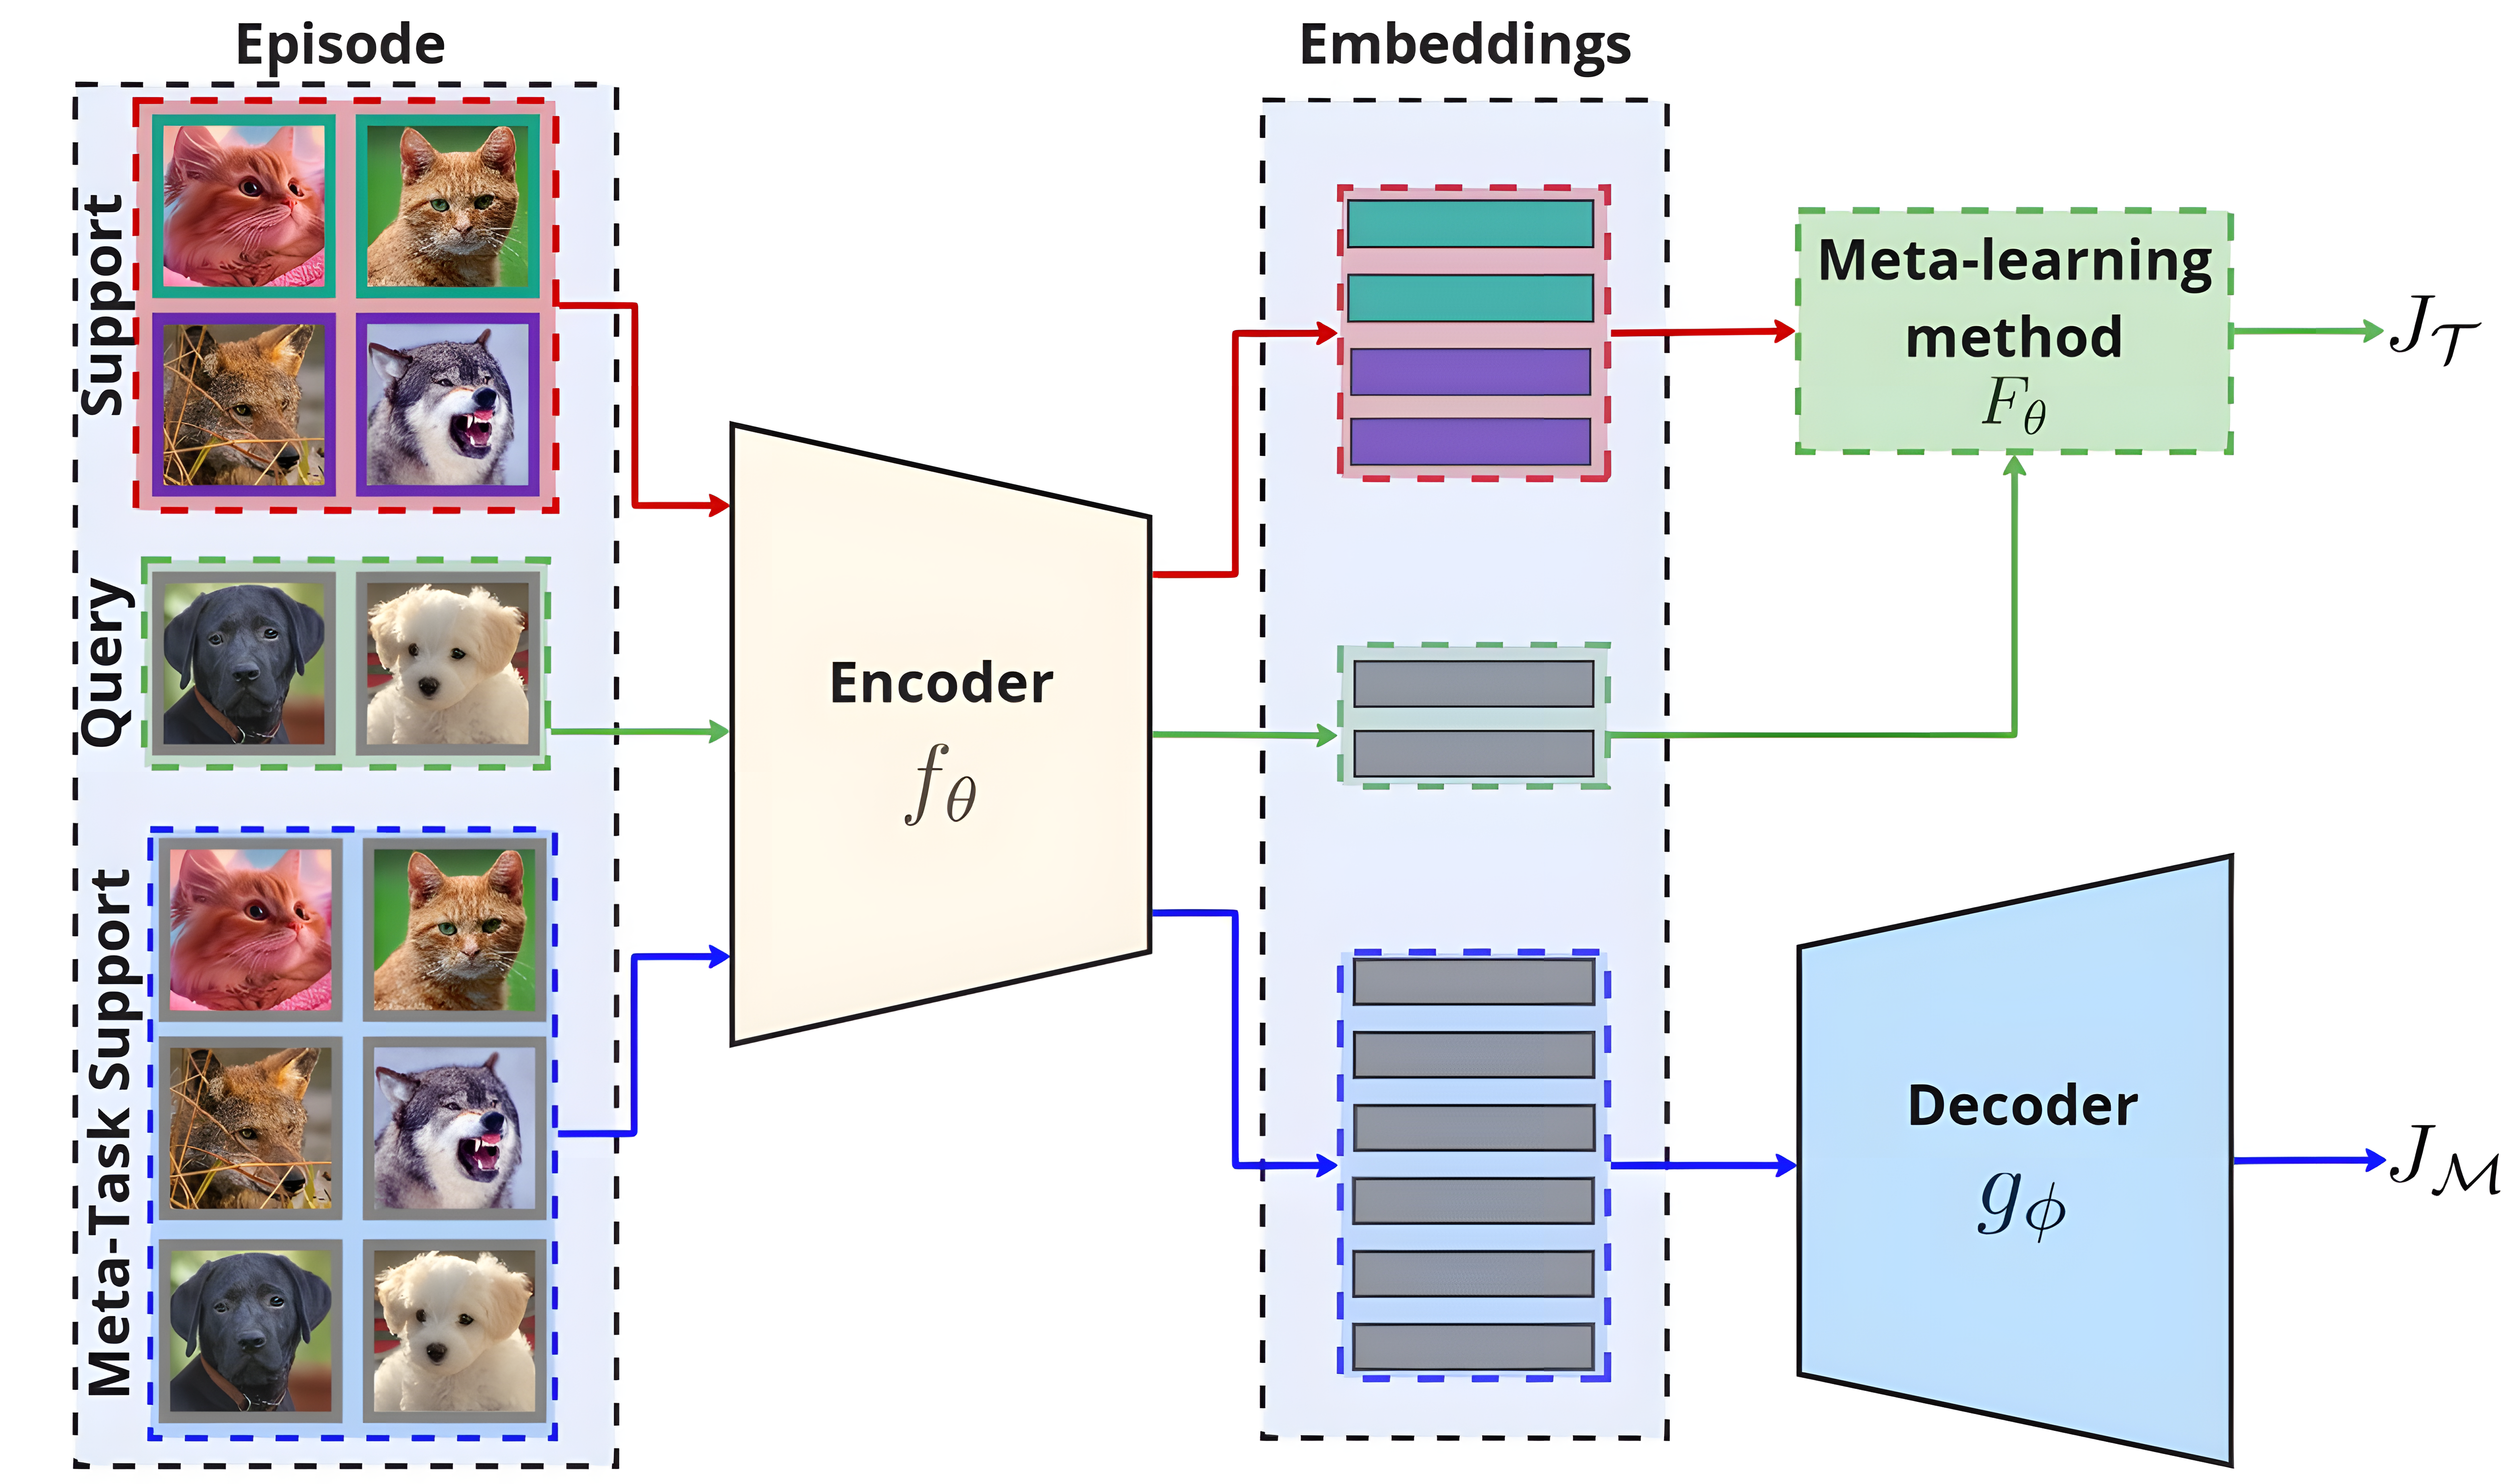
\includegraphics[width=\linewidth]{FIGURES/metatask/meta-tasks.png}   \caption{Detailed architecture of the Task-Decoder within the Meta-Task framework. The Meta-Task support set consists of unlabeled copies of support and query samples, which are fed into an encoder \( f_{\theta} \) to produce feature embeddings. These embeddings serve two key functions: (1) they are passed to a decoder \( g_{\phi} \) to reconstruct the input images, aiding in the learning of rich, meaningful representations, and (2) they are used to generate the meta-learning method ($F_{\theta}$) for query image classification. The model optimizes two objectives: classification loss (\( J_{\mathcal{T}} \)) and reconstruction loss (\( J_{\mathcal{M}} \)), each with a dedicated backpropagation step. The overall training loss is \( J_{\mathcal{T}} + \lambda J_{\mathcal{M}} \), balancing both classification accuracy and representation learning. For a broader application, the decoder \( g_{\phi} \) could be replaced by one or more neural networks that solve various unsupervised tasks.}

   \label{fig:1}
\end{figure}

\subsection{Related Work}


This section briefly reviews the relevant literature on meta-learning and regularization issues. Regularization techniques have been developed to improve the generalization ability of meta-learning models. These techniques can be broadly classified into four specialized regularization techniques for meta-learning. 1. Explicit Regularization (ER) \cite{rajeswaran2019imaml,mrmaml,pan2021meta,wang2023improving}, 2. Episode Augmentation Regularization (EAR) \cite{yamaguchi2023regularizing, shu2023dac}, 3. Task Augmentation Regularization (TAR) \cite{yao2021meta,yao2021improving,rajendran2020meta}, 4. Adversarial Task Upsampling (ATU) \cite{wu2022adversarial}. 

The ER methods impose explicit regularization terms on the meta-learning update, such as Meta-Learning with Implicit Gradients (iMAML) \cite{rajeswaran2019imaml}, Meta-Learning without Memorization (MR-MAML) \cite{mrmaml}, and their combinations or extensions \cite{pan2021meta, wang2023improving}. These methods directly constrain the model optimization process, aiming to improve the generalization performance of meta-learning models. For instance, minimax-meta regularization \cite{wang2023improving}
combines two types of regularizations at the inner and outer levels to enhance the generalization performance of bi-level meta-learning.

The EAR approach controls the meta-training by modifying individual tasks through noise or mixup \cite{yamaguchi2023regularizing, shu2023dac}. By expanding the amount of training data available for sampling, data augmentation supports various aspects of the meta-learning pipeline. It can be applied to support data in the inner loop of fine-tuning and enlarge the pool of evaluation data to be sampled during training. 

TAR methods generate new tasks by interpolating between or augmenting existing tasks \cite{yao2021meta, rajendran2020meta}, aiming to expand the task distribution for more robust generalization. For instance, methods such as MetaMix \cite{chen2021metamix}, and Channel Shuffle \cite{yao2021improving} have been proposed to increase the dependence of target predictions on the support set and provide additional knowledge to optimize model initialization. ProtoDiff \cite{du2023protodiff} enhances prototypical networks through a task-guided diffusion process; by generating synthetic features conditioned on the task, ProtoDiff \cite{du2023protodiff} augments the support set and improves the robustness of prototypes, significantly boosting classification performance. Additionally, the ATU approach \cite{wu2022adversarial} seeks to generate tasks that match the true task distribution by maximizing an adversarial loss, thereby improving meta-testing performance and the quality of upsampled tasks. These task augmentation techniques are designed to enhance the generalization capability of meta-learning models by effectively expanding the task distribution and mitigating overfitting during meta-training.

Recent works like Meta-Baseline \cite{chen2021metamix} have advanced few-shot learning by bridging transfer learning and meta-learning through pre-training feature extractors on base classes before few-shot fine-tuning, demonstrating that high-quality feature representations can sometimes eliminate the need for complex meta-learning algorithms. However, in contrast to Meta-Baseline's reliance on large-scale pre-training and ProtoDiff's \cite{du2023protodiff} computationally intensive task-guided diffusion models, our method learns robust embeddings during meta-training itself, making it more feasible for resource-constrained environments while remaining computationally efficient and method-agnostic.

In contrast to these methods, our proposed framework aims to regularize meta-learning tasks by introducing Meta-Tasks—auxiliary tasks designed to refine hidden representations without relying on extensive pre-training or synthetic data generation. Table \ref{tab:meta_learning_comparison} summarizes the key differences between various methods and our approach. We integrate an unsupervised autoencoder, specifically the Task-Decoder, directly within the meta-learning framework to provide continuous, unsupervised regularization during training. This helps prevent overfitting and improves generalization in an end-to-end manner.

By treating regularization as a learnable task, our framework enhances adaptability and generalization capabilities in a lightweight manner. It is suitable for a broader range of real-world applications where computational resources and labeled data are limited.

Meta-Task distinguishes itself from prior FSL approaches by introducing a learnable, task-specific regularization strategy that dynamically adapts to each task without modifying the underlying FSL architecture. Unlike LEO and iMAML, which focus on optimizing meta-initialization and gradient regularization, Meta-Task directly integrates into the optimization process through a parameterized neural layer $\phi$, learning task-adaptive constraints rather than enforcing fixed optimization heuristics. Unlike Wertheimer et al. \cite{wertheimer2021few} and Nag et al. \cite{nag2023reconstruction}, which utilize reconstruction-based self-supervision, our method does not rely on reconstruction loss. Furthermore, unlike Gidaris et al. \cite{gidaris2019boosting}, which introduces auxiliary tasks, Meta-Task requires neural layer $\phi$, instead only relying on better updates using self-supervised or semi-supervised tasks.

Our comprehensive experiments focus on fundamental meta-learning models (Prototypical Networks, MAML, MetaOptNet, and P$>$M$>$F~\cite{pmf}) that represent diverse approaches in the field. While some baseline comparisons were conducted with adjusted experimental settings (reduced batch sizes, modified query shots, etc.) due to computational constraints, our results consistently demonstrate the effectiveness of our Meta-Task framework across different meta-learning paradigms, validating its method-agnostic nature and broad applicability.

\begin{table}[ht]
\centering
\resizebox*{0.75\textwidth}{!}{
\begin{tabular}{lccccc}
\toprule
\textbf{Method} & \textbf{Category} & \textbf{Method-Agnostic} & \textbf{Complexity} \\
\midrule
\textbf{iMAML} \cite{imaml} & ER & No & High
\\
\textbf{MR-MAML} \cite{mrmaml} & ER & No & High \\ 
\textbf{Minimax-Meta} \cite{wang2023improving} & ER & No & Low \\
\textbf{DAC-MR} \cite{shu2023dac} & EAR & Yes & Medium \\
\textbf{MetaMix} \cite{chen2021metamix} & EAR & Yes & Medium \\
% \textbf{Channel Shuffle} \cite{yao2021improving} & TAR & Yes & Low \\
\textbf{ProtoDiff} \cite{du2023protodiff} & TAR & No & High \\
\textbf{ATU} \cite{wu2022adversarial} & TAR & Yes & High \\
\textbf{LEO} \cite{rusu2018meta} & ER & No & High \\
\textbf{Task-Decoder (Ours)} & \textbf{MTR} & \textbf{Yes} & \textbf{Medium} \\
\bottomrule
\end{tabular}
}
\caption{Comparison of meta-learning regularization methods. The table compares various meta-learning regularization techniques by category, method-agnostic capability, and computational complexity. Categories include Explicit Regularization (ER), Episode Augmentation Regularization (EAR), Task Augmentation Regularization (TAR), and our proposed Meta-Task Regularization (MTR).}
\label{tab:meta_learning_comparison}

\end{table}

\subsection{Meta-Task Framework}\label{sec:approach}
In this section, we introduce our proposed Meta-Task Framework, a novel approach that enhances generalization by integrating learnable Meta-Tasks as a form of regularization. By treating regularization itself as a learnable task, our framework encourages the model to develop richer and more robust feature representations. The framework is method-agnostic and can be seamlessly integrated with existing FSL models, such as Prototypical Networks and MAML. In the following subsections, we detail the components of the framework, including the Task-Decoder, the problem formulation, and the theoretical justification for its effectiveness.

Our framework extends MAML \cite{maml} by introducing regularization as a "learnable Meta-Task", enabling unsupervised task integration during meta-training without requiring additional data. The following subsections detail the implementation and theoretical foundations of our contributions:

\begin{itemize}
\item \textbf{Task-Decoder:} We introduce an unsupervised autoencoder architecture that implements our learnable regularization concept by reconstructing input images from their embeddings, proving its effectiveness in enriching feature representations.
\item \textbf{Problem Formulation:} We present the mathematical framework that enables the integration of unsupervised auxiliary tasks with existing FSL methods, demonstrating how our approach remains method-agnostic through separable loss functions.
\item \textbf{Theoretical Analysis:} We provide theoretical justification for our framework's convergence properties and establish how the joint optimization of primary and Meta-Tasks enhances generalization capabilities.
\end{itemize}

\subsubsection{Task-Decoder}

At the core of our Meta-Task Framework is the Task-Decoder (Figure \ref{fig:1}), an unsupervised learning component designed to enhance the embedding space by reconstructing input images from their embeddings. The Task-Decoder employs an autoencoder architecture, where the encoder \( f_{\theta} \) maps the input images to a latent embedding space, and the decoder \( g_{\phi} \) reconstructs the images from these embeddings.

By encouraging the embeddings to retain sufficient information for accurate reconstruction, the Task-Decoder prevents the encoder from focusing solely on discriminative features that may not generalize well. This leads to richer and more robust feature representations, ultimately improving the model's performance on unseen tasks.

The Task-Decoder operates in parallel with the primary few-shot learning model, processing the same inputs and contributing to the overall learning objective through its reconstruction loss.

\subsubsection{Problem Formulation}

Let the Meta-Task $\mathcal{M}$ denote the Task-Decoder, and our meta-learning method $F$ be Prototypical Networks. We define the encoder network \( f_{\theta} \) parameterized by \( \theta \), and \( g_{\phi} \) represent the decoder network parameterized by \( \phi \). 

For a given query sample \( x\in\mathcal{Q} \) and its true class \( y \) belonging to task $\mathcal{T}$, the Prototypical Network $F_{\theta}$ computes class prototypes using support set $\mathcal{S}$ and classifies $x$ based on the closest prototype to the embedding $f_{\theta}$.

\noindent
\textbf{Primary Task Loss:} The probability of \( x \) belonging to class \( n \) is:

\begin{equation} p_{\theta}(y={n} \mid x) = \frac{\exp\left(-d\left(f_{\theta}(x), c_{{n}}\right)\right)}{\sum_{k=1}^{N} \exp\left(-d\left(f_{\theta}(x), c_k\right)\right)}, \end{equation}
where $N$ is the number of tasks in the episode, \( c_n \) is the prototype of class \( n \) and \( d(\cdot, \cdot) \) denotes the Euclidean distance. The classification loss is then:

\begin{equation}
J_{\mathcal{T}}(x, \theta) = -\log p_{\theta}(y = n \mid x).
\end{equation}

\noindent
\textbf{Meta-Task Loss:} The Task-Decoder aims to reconstruct \( x \) from \( f_{\theta} \), with the reconstruction loss defined as:

\begin{equation}
J_{\mathcal{M}}(x, \theta, \phi) = \left\| g_{\phi}(f_{\theta}(x)) - x \right\|^2.
\end{equation}

\noindent
\textbf{Combined Loss Function:} The total loss for a sample \( x \) is a weighted sum of the primary task loss and the Meta-Task loss:

\begin{equation}
J(x, \theta) = J_{\mathcal{T}}(x, \theta) + \lambda J_{\mathcal{M}}(x, \theta, \phi),
\end{equation}
where \( \lambda \) is a hyperparameter balancing the two losses or the learning rate for the Meta-Task update.

\noindent
\textbf{Optimization:} The model parameters \( \theta \) and \( \phi \) are optimized jointly over all tasks and samples. For a given task $\mathcal{T}$, the overall loss is calculated by summing the combined losses over all query samples:

\begin{equation}\label{eq:task_loss}
J_{\mathcal{T}}(\theta) = \sum_{x \in \mathcal{T}} J_{\mathcal{T}}(x, \theta). 
\end{equation}

During meta-training, we sample a batch of tasks $\{\mathcal{T}_i\}^L_{i=1}$. The total loss across all tasks in an episode is:

\begin{equation}\label{eq:overall_loss_separate}
J(\theta) = \sum_{i=1}^{L} \left(J_{\mathcal{T}_i}(\theta) + \lambda J_{{\mathcal{M}_i}}(\theta, \phi)\right).
\end{equation}

By minimizing this combined loss, the model learns embeddings that are both discriminative for classification and informative for reconstruction, enhancing generalization across tasks. The full algorithm of the Task-Decoder integration is provided in Algorithm~\ref{alg:task_decoder}.

We define tasks and Meta-Tasks as separable if their loss functions can be computed independently and summed without including interaction terms. This structure allows us to optimize each component separately while still contributing to the overall objective. If the regularization term is separable (as in our case with the autoencoder), we can simplify \eqref{eq:overall_loss_separate} as
\begin{equation}\label{eq:9}
J(\theta) = \sum_{i=1}^{L} J_{\mathcal{T}_i}(\theta) +\lambda\sum_{i=1}^{L}J_{{\mathcal{M}_i}}(\theta,\phi).
\end{equation}

If each task may have multiple or no Meta-Tasks attached, the overall loss function generalizes to:
\begin{equation}\label{eq:10}
J(\theta) = \sum_{i=1}^{L} J_{\mathcal{T}_i}(\theta) +\lambda\sum_{r=1}^{R}J_{{\mathcal{M}_r}}(\theta,\phi),
\end{equation}
where $R$ is the total number of regularizers applied to the model.

\subsubsection{Justification}

Our Meta-Task framework provides unique theoretical guarantees, distinguishing it from existing regularization approaches. In Equations \eqref{eq:9} and \eqref{eq:10}, we demonstrated that incorporating auxiliary tasks into training effectively reformulates the FSL paradigm to a new FSL setting with a combined distribution of primary tasks and Meta-Tasks, denoted as 
$\mathcal{T}'$. This reformulation allows the overall training objective to be expressed as a sum over $L+R$ tasks, preserving the structure necessary for standard FSL optimization techniques.

When using MAML as the FSL method, based on convergence guarantees proven in literature~\cite{wang2022global}, our approach converges to an optimal set of parameters for $\mathcal{T}'$. Since the Meta-Tasks are carefully designed to enhance generalization, this optimal parameter set enables the model to generalize effectively across both primary tasks and Meta-Tasks. The convergence of $\phi$ to its global optima further ensures that the learned embeddings retain the essential information necessary for both classification and reconstruction. This joint optimization ($\theta$) constructs a globally optimal representation space, improving overall model performance on unseen tasks by reducing generalization error.

A critical advantage of Meta-Task is the separability of the primary and auxiliary tasks. Since their loss functions can be computed independently, optimization can proceed efficiently, with each task contributing to the overall objective. This design simplifies the optimization process and supports convergence to a global optimum, as the auxiliary tasks act as an implicit regularizer, reducing overfitting by penalizing non-generalizable embeddings.

A rigorous mathematical proof is more challenging for FSL methods beyond MAML. However, as all FSL methods aim to optimize parameters that generalize across task distributions with limited examples, it is reasonable to infer that our approach improves generalization capabilities, as demonstrated in the results section. In the supplementary material, we provide additional experiments, including visualizations of reconstructed features, to empirically validate how Meta-Task enhance embedding quality and task generalization.

\begin{remark}{The proposed regularization approach is method-agnostic and can be applied to any FSL learning method.} \end{remark}
\begin{remark}{Equations \eqref{eq:9}, \eqref{eq:10} hold only if tasks and Meta-Tasks are separable or independent.}
\end{remark}
\begin{remark}{The use of autoencoders is because autoencoders can be used with any type of data, are easy to use, and are flexible in architecture.}
\end{remark}

\begin{algorithm}[t]
  \caption{Meta-Tasks: Task-Decoder}
  \label{alg:task_decoder}
  \begin{enumerate}
      \item \textbf{Require:} Distribution over tasks $p(\mathcal{T})$; \\
      \item \textbf{Require:} embedding network $f_{\theta}$; \\
      \item \textbf{Require:} decoder network $g_{\phi}$; \\
      \item \textbf{Require:} learning rates $\alpha$, $\lambda$; 
      \item \textbf{Require:} meta-learning method $F$ (e.g., Prototypical Networks); 
      \item \textbf{Require:} classification loss $J_{\mathcal{T}}(x, \theta)$;
      \item \textbf{Require:} reconstruction loss $J_{\mathcal{M}}(x, \theta, \phi) = \| g_{\phi}(f_{\theta}(x)) - x \|^2$ \\
      \item Randomly initialize $\theta$ and $\phi$
      \item \textbf{while} not done \textbf{do}
      \begin{enumerate}
          \item Sample support set $\mathcal{S} \sim p(\mathcal{T})$
          \item Sample query set $\mathcal{Q} \sim p(\mathcal{T})$
          \item Compute reconstruction loss: \\
          $J_{\mathcal{M}}(\theta, \phi) \leftarrow \frac{1}{|\mathcal{S} \cup \mathcal{Q}|} \sum_{x \in \mathcal{S} \cup \mathcal{Q}} J_{\mathcal{M}}(x, \theta, \phi)$
          \item Use support set $\mathcal{S}$ and embedding network $f_{\theta}$ to obtain meta-learning method $F_{\theta}$
          \item Compute classification loss on query set: \\
          $J_{\mathcal{T}}(\theta) \leftarrow \frac{1}{|\mathcal{Q}|} \sum_{x \in \mathcal{Q}} J_{\mathcal{T}}(x, F_{\theta})$
          \item Update embedding network parameters: \\
          $\theta \leftarrow \theta - \alpha \nabla_{\theta} \left( J_{\mathcal{T}}(\theta) + \lambda J_{\mathcal{M}}(\theta, \phi) \right)$
          \item Update decoder parameters: \\
          $\phi \leftarrow \phi - \lambda \nabla_{\phi} J_{\mathcal{M}}(\theta, \phi)$
      \end{enumerate}
      \item \textbf{end while}
  \end{enumerate}
  \end{algorithm}


\subsection{Experiments and Results}\label{sec:results}

In this section, we conduct comprehensive experiments to validate the effectiveness of our proposed {Meta-Task} framework in enhancing generalization and mitigating overfitting in few-shot learning. Our objectives are to: 
\begin{enumerate} 
\item Demonstrate that incorporating Meta-Tasks as auxiliary regularization improves model generalization to both seen and unseen tasks.
\item Validate that leveraging both labeled and unlabeled data through an unsupervised autoencoder refines hidden representations.
\item Showcase the method-agnostic applicability of {Meta-Task} across various FSL settings and its practical efficiency in resource-constrained scenarios. 
\end{enumerate}
  
We begin by outlining the experimental setup, including datasets, model architectures, and implementation specifics. Following this, we present our results along with a comprehensive analysis of our findings, focusing on the impact of the {Meta-Task} framework on performance, convergence speed, and variance reduction.
  
\subsubsection{Datasets}
  
We evaluated the proposed {Meta-Task} framework on three standard benchmarks commonly used in few-shot learning:

\noindent
\textbf{MiniImageNet}~\cite{mini-imagenet}: This dataset consists of 100 classes selected from ImageNet, with 600 images per class resized to $84 \times 84$ pixels. It is divided into 64 training, 16 validation, and 20 test classes, ensuring that test classes are entirely disjoint from training classes for robust evaluation of generalization capabilities.

\noindent
\textbf{TieredImageNet}~\cite{ren2018meta}: A larger and more challenging dataset comprising 608 classes organized into 34 high-level categories, providing semantic diversity. It includes 351 training, 97 validation, and 160 test classes, with images resized to $84 \times 84$ pixels. Its hierarchical structure makes it suitable for evaluating models' ability to generalize across different levels of abstraction.

\noindent
\textbf{FC100}~\cite{oreshkin2018tadam2}: Derived from the CIFAR-100 dataset, FC100 contains 100 classes, each with 600 images resized to $32 \times 32$ pixels. The dataset is split into 60 training, 20 validation, and 20 test classes. It presents unique challenges due to low-resolution images and high intra-class variability, making it an excellent benchmark for assessing model robustness.
  
These datasets offer diverse and challenging scenarios for few-shot learning, enabling us to thoroughly evaluate the generalization capabilities of the {Meta-Task} framework.
  
\subsubsection{Methods}
  
To demonstrate the method-agnostic nature of our approach, we integrated the {Meta-Task} framework with four few-shot learning models:

\noindent
\textbf{Prototypical Network (PN)} \cite{snell2017prototypical}: Utilizes a ResNet-50 \cite{resnet-code} backbone for feature extraction. It computes class prototypes in the embedding space, classifying query samples based on their distances to these prototypes.

\noindent
\textbf{MAML}~\cite{maml}: Employs a four-layer ConvNet architecture aiming to find initial model parameters that can be quickly adapted to new tasks with minimal gradient updates.

\noindent
\textbf{MetaOptNet}~\cite{lee2019metaoptnet}: Uses a ResNet-12 backbone and incorporates differentiable convex optimization layers for efficient classification, seamlessly integrating with our {Meta-Task} framework.

\noindent
\textbf{P$>$M$>$F} \cite{pmf}: Uses DINO\cite{dino} framework as its backbone. Like PN, it computes class prototypes in the embedding space. It classifies query samples based on their distances to these prototypes but with the added benefit of leveraging pre-trained transformer-based feature extraction.

In our {Meta-Task} framework, we introduced a Task-Decoder employing an unsupervised autoencoder to reconstruct input images from their embeddings. The decoder mirrors the encoder architecture used in the backbone models. This process leverages both labeled and unlabeled data (support and query sets), refining the hidden representations and mitigating overfitting.

For the autoencoder architecture, we experimented with different configurations to assess the impact of the Task-Decoder's depth on performance. Specifically, we used both shallow and deep autoencoders, with parameters ranging from 75K to 250K. The shallow autoencoder consists of two convolutional layers, while the deep autoencoder includes four convolutional layers. This allowed us to analyze how the complexity of the Task-Decoder affects the overall performance.

We trained all models using the Adam optimizer with learning rates set to $1 \times 10^{-4}$ for the encoder and classifier, and $1 \times 10^{-6}$ for the Task-Decoder. Each model was trained over 50,000 episodes using 5-way 1-shot and 5-way 5-shot scenarios. The query size was maintained at 15 for both training and evaluation phases. To enhance model robustness, we applied standard data augmentation techniques, including random cropping, horizontal flipping, and color jittering.

Furthermore, we investigated the effect of using multiple autoencoders per task by associating different autoencoders with specific layers of the encoder network. However, we found that using a single autoencoder provided a good trade-off between performance improvement and computational overhead. The complete source code and results for this paper can be found in the following GitHub repository: \href{https://github.com/woreom/meta-learning}{https://github.com/woreom/meta-learning}.
  

\begin{figure}
  
  \centering
    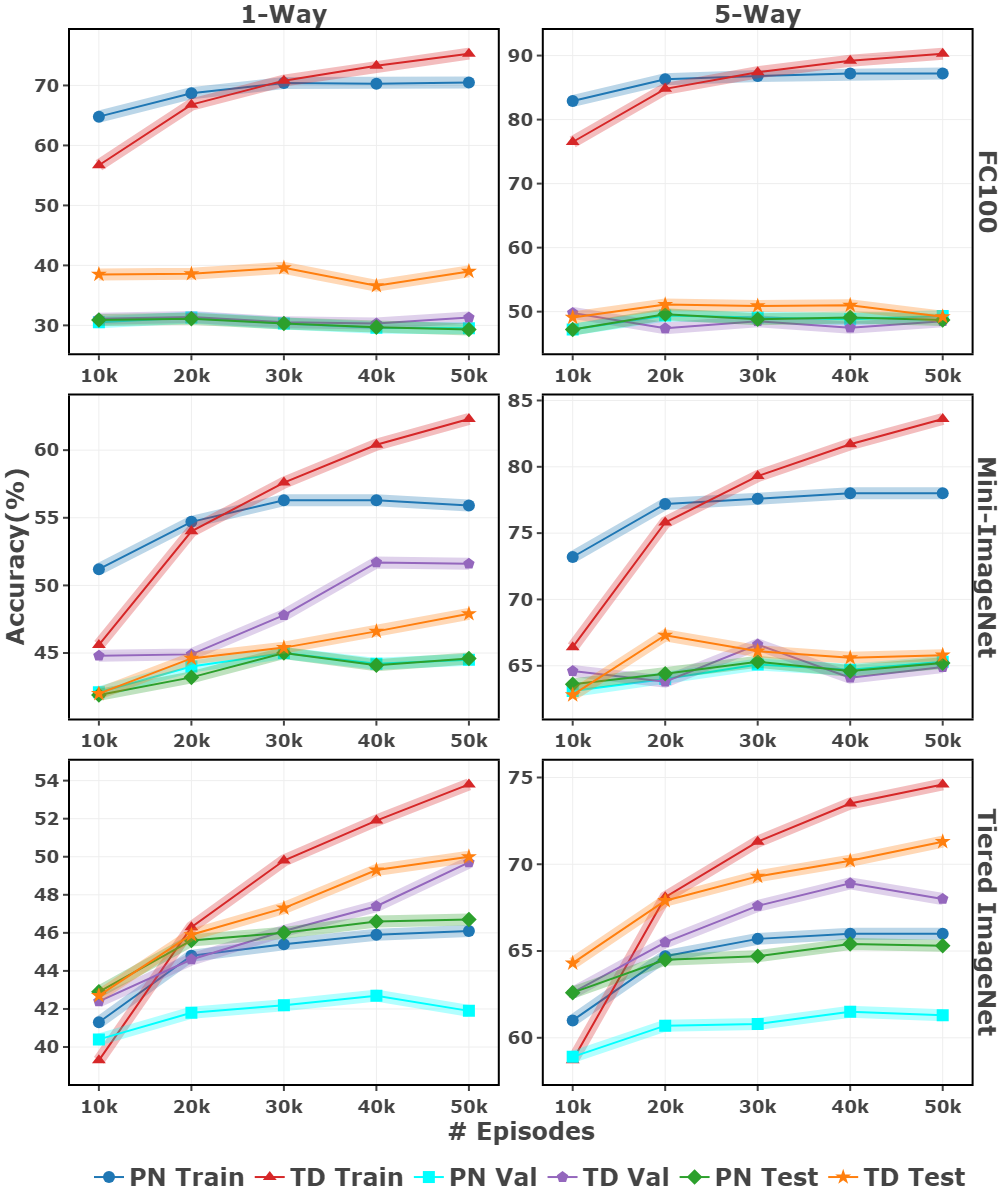
\includegraphics[width=0.9\linewidth]{FIGURES/metatask/acc_2.png}
    \caption{Accuracy curves for Prototypical Networks (PN) and Task-Decoder (TD) across different datasets, plotted against the number of episodes.}
    \label{fig:5}
\end{figure}

\begin{figure}
    \centering
     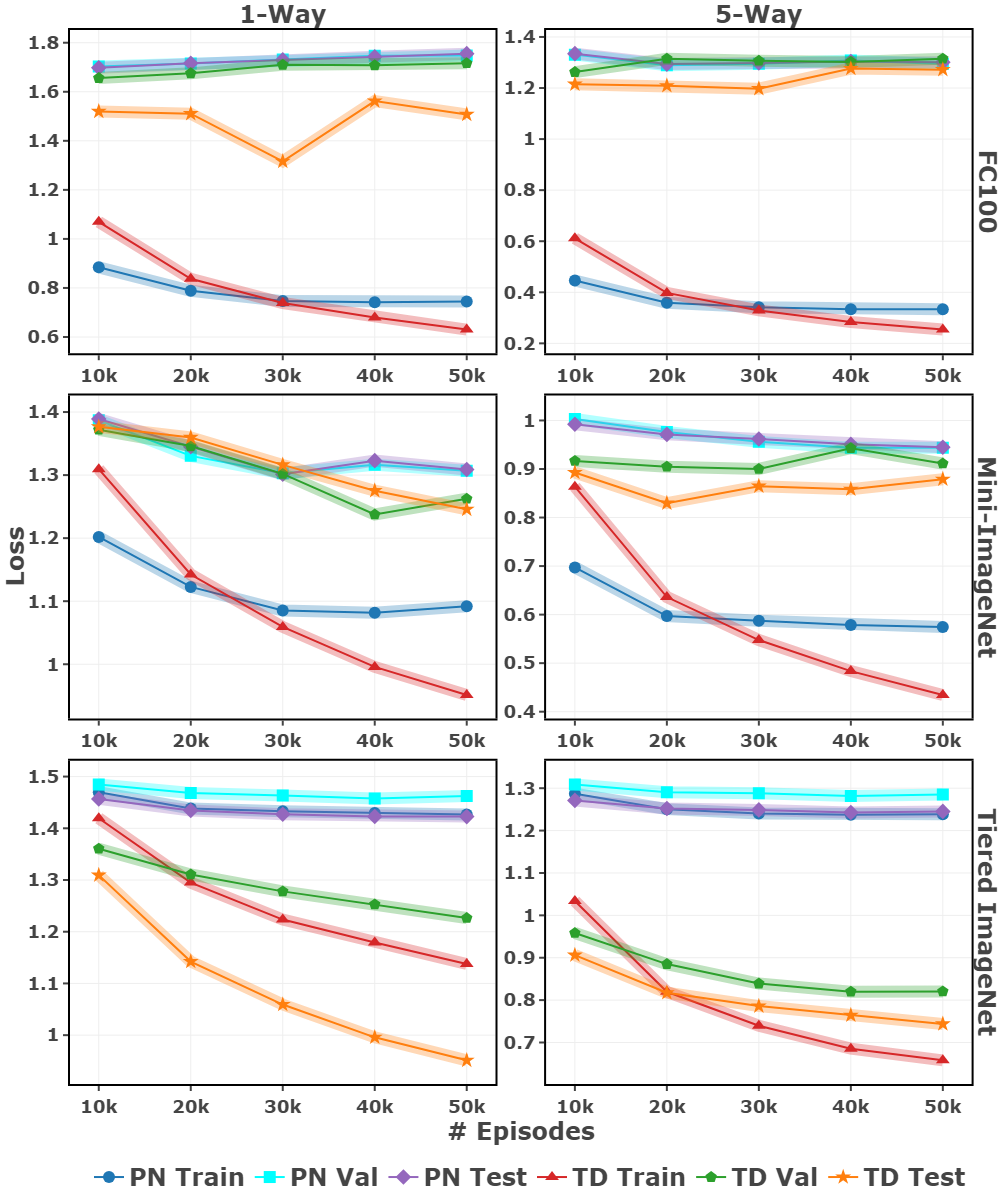
\includegraphics[width=0.9\linewidth]{FIGURES/metatask/loss_2.png}
     \caption{Loss curves for Prototypical Networks (PN) and Task-Decoder (TD) across different datasets, plotted against the number of episodes.}
     \label{fig:4}
  \end{figure}

  \begin{table}[!htbp]
    \centering
    \resizebox*{!}{0.4\linewidth}{
    \begin{tabular}{ll|cccc}
                                                    &                    & \multicolumn{2}{c}{MiniImageNet}                                        & \multicolumn{2}{c}{TieredImageNet}                                          \\
    Method                                         & Backbone           & \multicolumn{1}{l}{5-way 1-shot(\%)} & \multicolumn{1}{l}{5-way 5-shot(\%)} & \multicolumn{1}{l}{5-way 1-shot(\%)} & \multicolumn{1}{l}{5-way 5-shot(\%)} \\
    \hline
    PN                           & ResNet18           & 45 ± 0.0                         & 65.2 ± 0.0                           & 46.6 ± 0.0                           & 65.4 ± 0.0                           \\
    \textbf{PN(TD)}              & ResNet18           & \textbf{47.9 ± 0.0}              & \textbf{66.1 ± 0.0}                  & \textbf{50 ± 0.0}                    & \textbf{71.3 ± 0.0}                  \\
    MAML                         & CNN                & 47.54                            & 62.23                                & -                                    & -                                    \\
    \textbf{MAML (TD)}           & Shallow CNN Decoder& \textbf{47.81}                   & \textbf{62.52}                       & -                                    & -                                    \\
    \textbf{MAML (TD)}           & CNN                & \textbf{47.67}                   & \textbf{63.01}                       & -                                    & -                                    \\
    Relation Networks\cite{sung2017learning}      & 64-96-128-256      & 50.44 ± 0.82                     & 65.32 ± 0.70                         & 54.48 ± 0.93                         & 71.32 ± 0.78                         \\
    R2D2\cite{bertinetto2018meta}        & 96-192-384-512     & 51.2 ± 0.6                       & 68.8 ± 0.1                           & -                                    & -                                    \\
    Transductive Prop Nets\cite{liu2018learning} & 96-192-384-512     & 55.51 ± 0.86                     & 69.86 ± 0.65                         & 59.91 ± 0.94                         & 73.3 ± 0.75                          \\
    SNAIL\cite{mishra2017simple}         & ResNet-12          & 55.71 ± 0.99                     & 68.88 ± 0.92                         & -                                    & -                                    \\
    AdaResNet\cite{munkhdalai2018rapid} & ResNet-12          & 56.88 ± 0.62                     & 71.94 ± 0.57                         & -                                    & -                                    \\
    TADAM\cite{oreshkin2018tadam2}      & ResNet-12          & 58.5 ± 0.30                      & 76.7 ± 0.30                          & -                                    & -                                    \\
    MetaOptNet                   & ResNet-12          & 61.23 ± 0.29                     & 77.14 ± 0.21                         & 63.10 ± 0.34                         & 78.58 ± 0.27                         \\
    \textbf{MetaOptNet (TD)}     & ResNet-12          & \textbf{61.35 ± 0.29}            & \textbf{77.3 ± 0.22}                 & \textbf{63.20 ± 0.34}                & \textbf{78.66 ± 0.27}                \\
    \textbf{P$>$M$>$F}           & IN1K,ViT-base       & \textbf{72.80 ± 0.0}             & \textbf{90.70 ± 0.0}                 & -                                    & -                                    \\
    \textbf{P$>$M$>$F(TD)}       & IN1K,ViT-base       & \textbf{74.10 ± 0.0}             & \textbf{92.30 ± 0.0}                 & -                                    & -                                    \\
    \hline
    \end{tabular}}
    \caption{Comparison of few-shot classification accuracies (\%) with 95\% confidence intervals on MiniImageNet and TieredImageNet datasets. Results are reported for 5-way 1-shot and 5-way 5-shot. `PN` and `TD` refer to Prototypical Networks and Task-Decoder, respectively.}
    \label{table:1}
  \end{table}


  \begin{table}[!htpb]
  \centering
  \resizebox*{!}{0.25\linewidth}{\begin{tabular}{l|cc}
                                                &  \multicolumn{2}{c}{FC100}                                                   \\
  Method                                         & \multicolumn{1}{l}{5-way 1-shot(\%)} & \multicolumn{1}{l}{5-way 5-shot(\%)} \\
  \hline & & \\
  PN                            & 31.1 ± 0.0                           & 49.6 ± 0.0                           \\
  \textbf{PN (TD)}  & \textbf{39 ± 0.0}                    & \textbf{51.1 ± 0.0}                  \\
  TADAM\cite{oreshkin2018tadam2}                  & 40.1 ± 0.4                           & 56.1 ± 0.4                           \\
  MetaOptNet                                     & 40.19 ± 0.25                         & 55.04 ± 0.26                         \\
  \textbf{MetaOptNet (TD)}             & \textbf{40.59 ± 0.26}                & \textbf{55.38 ± 0.25}                \\
  \hline
  \end{tabular}}
  \caption{Comparison of few-shot classification accuracies (\%) with 95\% confidence intervals on the FC100 dataset \cite{oreshkin2018tadam2}. Results are reported for 5-way 1-shot and 5-way 5-shot settings. `PN' and `TD' refer to Prototypical Networks and Task-Decoder, respectively.}
  \label{table:2}
  \end{table}

\subsubsection{Performance Evaluation}

Our experimental results demonstrate that the Meta-Task framework consistently outperforms baseline models across all datasets and settings, achieving higher accuracy with significantly fewer training episodes. For example, as shown in Figure~\ref{fig:5}, TD enables higher test accuracy within 20k episodes, whereas PN Test fails to achieve the same even after 50k episodes. Similarly, in Table~\ref{table:1}, TD P$>$M$>$F reaches 92.30\% accuracy in 3k episodes compared to P$>$M$>$F's 90.70\% after 4k episodes.

These results highlight the framework's efficiency in leveraging a small number of additional parameters to enhance generalization while reducing computational overhead. By introducing Meta-Tasks, the learning process is effectively regulated, eliminating the need for extensive parameter tuning or large-scale episodic training. This makes the Meta-Task framework both lightweight and practical for real-world applications. Further details on are provided in Table~\ref{table:1} and Table~\ref{table:2}.
  
\textbf{Prototypical Network Results}
Table~\ref{table:1} presents our experimental results on MiniImageNet and TieredImageNet, where our proposed method, the Task-Decoder, demonstrates significant performance improvements over the baseline Prototypical Networks. Specifically, on TieredImageNet in the 5-way 5-shot setting, our approach achieved an increase from 65.4\% to 71.3\% in test set accuracy, reflecting a substantial 5.9\% absolute improvement. This gain indicates superior meta-generalization capabilities of our method.

In the 5-way 1-shot scenario, the Task-Decoder improved accuracy from 46.6\% to 50\% on TieredImageNet, highlighting its efficacy in scenarios with extremely limited data. These consistent improvements across different datasets and settings demonstrate the robustness and effectiveness of our approach.

\textbf{MAML Results}
Table~\ref{table:1} also showcases the performance of the {Task-Decoder} integrated with MAML. Our method outperforms the baseline MAML by an average of 0.48\% in the 5-way 1-shot setting and 0.78\% in the 5-way 5-shot setting on MiniImageNet. Although the absolute improvements are modest, they demonstrate the effectiveness of the {Task-Decoder} in enhancing the adaptability of MAML.
  
To examine the impact of the {Task-Decoder's} architecture ($\phi$) on generalization, we trained MAML using two different{Task-Decoders}: a shallow decoder with 75K parameters and a deeper decoder with 250K parameters. Interestingly, the shallow decoder excelled in the 5-way 1-shot task, suggesting that deeper models are not always superior when data is scarce. In contrast, the deeper decoder performed better with more shots, highlighting the importance of model depth in specific contexts. This indicates that the Task-Decoder and its Meta-Task extensions can be effective even with a shallow network, which is beneficial in resource-constrained environments.
  
It's important to note that MAML requires the computation of second derivatives during optimization. However, to remain consistent with our claim of a method-agnostic framework, we chose to use a first-order approximation for the Task-Decoder's optimization. This decision avoids the computational overhead associated with second-order derivatives but may introduce approximation errors. Another limitation may stem from the inherent difficulties of optimizing the learning rate in MAML, which is complicated by the need for careful tuning due to its sensitivity to hyperparameters. While using the same learning rate as the Prototypical Networks simplifies comparisons, it likely constrained MAML's overall performance. These factors suggest that further optimization and fine-tuning could enhance the benefits of integrating the Task-Decoder with MAML.
  
textbf{MetaOptNet Results}
The results presented in Table~\ref{table:1} indicate that integrating the Task-Decoder with MetaOptNet \cite{lee2019meta} leads to modest but consistent performance improvements, with an average accuracy increase of 0.12\% in the 5-way 1-shot setting and 0.16\% in the 5-way 5-shot setting on MiniImageNet. While these gains are not as pronounced as those observed with other methods, they underscore the potential of the Task-Decoder to enhance performance even in well-optimized frameworks like MetaOptNet.

We attribute the smaller improvements to MetaOptNet's distinctive training setup, where variations in batch size and the number of shots significantly impact model performance. Due to hardware limitations, we reduced the batch size and the number of training shots, which may have constrained the performance gains. These findings suggest that further hyperparameter optimization, such as adjusting batch size or learning rate, could yield more substantial improvements.

\textbf{P$>$M$>$F Results}

Due to the pre-trained nature of the encoder, we implemented a custom scheduler to align TD's optimization. Additionally, hardware constraints necessitated deviations from the original hyperparameters, such as reducing image sizes and query shots, which may have influenced the observed improvements. Despite these constraints, TD achieved a notable 1.45\% performance increase, demonstrating its flexibility and adaptability to transformer-based methods under constrained conditions.
  
\subsubsection{Regularization Improvements}

Figure~\ref{fig:5} illustrates that our method achieves higher accuracy more quickly during all training, validation, and testing phases compared to the baseline, which demonstrates faster convergence. Additionally, Figure~\ref{fig:4} illustrates that the loss associated with our method decreases more rapidly and consistently remains lower throughout the training process across all training, validation, and test sets. The Task-Decoder achieves a mean loss of 1.23 with a variance of 0.001, whereas the baseline has a mean loss of 1.3 and a variance of 0.0002. This indicates more efficient learning and improved generalization.
  
To address concerns regarding implementation specifics, we have provided detailed information about the hyperparameters, training times, and autoencoder architectures in the supplementary material. We also conducted ablation studies to analyze the effect of different autoencoder architectures and the use of multiple autoencoders per task. The results indicate that while deeper autoencoders can provide marginal performance gains, the computational overhead increases significantly. Therefore, a single, appropriately sized autoencoder strikes a good balance between performance and efficiency.
  
\subsection{Conclusion}

In this paper, we introduced the {\textbf{Meta-Task}} framework, a method-agnostic approach for regularization in few-shot learning (FSL) that leverages Meta-Tasks as auxiliary tasks with a set of parameters to mitigate overfitting. Theoretically, we demonstrated that our approach achieves global optima with strong generalization across tasks. Empirically, we validated its efficacy through the {\textbf{Task-Decoder}} Meta-Task, which significantly improved performance on MiniImageNet and TieredImageNet benchmarks, achieving faster convergence and reduced generalization error with minimal hyperparameter tuning. Overall, our findings highlight the potential of the {{Meta-Task}} framework to improve FSL models, suggesting that even minor adjustments can lead to significant benefits and encourage further exploration of Meta-Task-based regularization in broader contexts.

\section{Overall Findings}

Across the three core tasks—BEpiC, MetaRep, and Meta-Task—this chapter systematically advances the state of generalization in few-shot learning by addressing complementary challenges in episode generation, representation learning, and regularization. These contributions collectively demonstrate Stage 2 of our wireless foundation model framework: enabling rapid task adaptation with minimal labeled data.

\textbf{BEpiC} introduced binary episodes to improve cross-domain generalization, addressing the challenge of distribution shift between meta-training and meta-test tasks. By simplifying episodes to binary classification problems, BEpiC encourages learning of domain-invariant representations that transfer more robustly across different task distributions. For wireless foundation models, this translates to better generalization across SNR regimes, channel conditions, and potentially unseen modulation families—reducing the brittleness of models trained on fixed task distributions.

\textbf{MetaRep} demonstrated that leveraging both labeled and unlabeled data through episodic representation learning significantly enhances meta-learning performance. By learning task-conditioned feature modulations, MetaRep adapts representations dynamically based on the support set, enabling more effective few-shot classification. This aligns with the foundation model principle of learning general-purpose representations that can be rapidly specialized—Meta-Rep shows how to modulate pre-trained features for specific tasks without extensive retraining.

\textbf{Meta-Task} introduced method-agnostic learnable regularization, showing that adaptive regularization strategies improve few-shot generalization across diverse meta-learning algorithms. This finding is critical for foundation models, which must be robust to various deployment scenarios. Meta-Task's approach of learning when and how to regularize based on task characteristics provides a principled mechanism for ensuring reliable adaptation regardless of the specific meta-learner or downstream application.

\textbf{Collectively}, these contributions demonstrate that enhancing generalization in few-shot learning requires a holistic approach: (1) designing episodes that expose the learner to meaningful task diversity (BEpiC), (2) leveraging both labeled and unlabeled data to learn robust, adaptable representations (MetaRep), and (3) integrating adaptive, learnable regularization mechanisms (Meta-Task). The empirical results consistently show that each method yields measurable improvements in accuracy, robustness, and data efficiency, and that their principles are broadly applicable across meta-learning paradigms.

\textbf{Foundation Model Implications:} This chapter establishes meta-learning as the critical adaptation layer (Stage 2) in our wireless foundation model framework. Given pre-trained representations from DenoMAE (Chapter 2, Stage 1), these meta-learning techniques enable rapid specialization to new modulation classification tasks with minimal labeled samples. The ability to adapt quickly with few examples is the hallmark of foundation models—distinguishing them from traditional supervised approaches. BEpiC, MetaRep, and Meta-Task collectively demonstrate that wireless signals can exhibit this rapid adaptation capability, bridging the gap between general-purpose pre-training and task-specific deployment. The next chapter (Chapter 4) explores semi-supervised learning as a practical training methodology, and Chapter 5 integrates these adapted representations with LLMs to enable true open-set recognition—completing the wireless foundation model vision.